\documentclass{VUMIFPSmagistrinis}
% \usepackage{algorithmicx}
% \usepackage{algorithm}
% \usepackage{algpseudocode}
\usepackage{amsfonts}
\usepackage{amsmath}
\usepackage{bm}
\usepackage{caption}
\usepackage{color}
\usepackage{float}
\usepackage{graphicx}
\usepackage{listings}
\usepackage{subfig}
\usepackage{wrapfig}

% Default settings for code listings
\lstset{frame=tb,
  language=scala,
  captionpos=b,
  aboveskip=3mm,
  belowskip=3mm,
  showstringspaces=false,
  columns=flexible,
  basicstyle={\small\ttfamily},
  numbers=none,
  numberstyle=\tiny\color{gray},
  %keywordstyle=\color{blue},
  %commentstyle=\color{dkgreen},
  %stringstyle=\color{mauve},
  frame=single,
  breaklines=true,
  breakatwhitespace=true
  tabsize=3
}

\renewcommand{\lstlistingname}{Kodo pavyzdys}

% Titulinio aprašas
\university{Vilniaus universitetas}
\faculty{Matematikos ir informatikos fakultetas}
\department{Programų sistemų katedra}
\papertype{Magistro baigiamasis darbas}
\title{Reaktyvus programavimas įvykių kaupimo sistemose}
\titleineng{Reactive Programming in Eventsourcing Systems}
\author{Žilvinas Kučinskas}
% \secondauthor{Vardonis Pavardonis}   % Pridėti antrą autorių
\supervisor{Viačeslav Pozdniakov}
\reviewer{prof. Rimantas Vaicekauskas}
\date{Vilnius – \the\year}

% Nustatymai
% \setmainfont{Palemonas}   % Pakeisti teksto šriftą į Palemonas (turi būti įdiegtas sistemoje)
\bibliography{bibliografija}

\begin{document}
\maketitle

%% Padėkų skyrius
% \sectionnonumnocontent{}
% \vspace{7cm}
% \begin{center}
%     Padėkos asmenims ir/ar organizacijoms
% \end{center}

\sectionnonumnocontent{Santrauka}

Įvykių kaupimo principu paremtose sistemose dažnai naudojamas komandų-užklausų atskyrimo principas. Kartu, šie principai leidžia kurti reaktyviąsias sistemas, apibrėžtas ``Reaktyvumo manifeste''. Tuo tarpu reaktyvus programavimas leidžia realizuoti reaktyviąsias programas komponavimo būdu, tai yra deklaratyviu stiliumi. Tokiu stiliumi kuriamos programos leidžia atskirti pagrindinę logiką į smulkesnes, lengviau suprantamas dalis. Darbe siekiama sukurti reaktyviojo programavimo programos sąsają, kuri leistų šiuos principus sujungti kartu užtikrinant sistemos atkuriamumą, našumą, reagavimą į įvykius kuriant įvykių kaupimo sistemos skaitymo modelį. Darbe naudojama ``Ruby'' programavimo kalbos sintaksė, parodomas aukšto lygmens architektūros modelis, įgyvendinamas ``Ruby on Rails'' programų kūrimo karkase, panaudojant modelio-kontrolieriaus-vaizdo projektavimo šabloną, reaktyvaus programavimo, įvykių kaupimo bei komandų-užklausų atsakomybių atskyrimo principus. Reaktyvūs filtravimo, transformacijos, srautų sujungimo bei imties mažinimo operatoriai leidžia atskirti dalį domeno logikos į smulkesnius, lengviau suprantamus bei palaikomus komponentus. Ši sąsaja lyginama su modelio-kontrolieriaus-vaizdo projektavimo šablono maršrutizatoriaus paskirtimi.

\raktiniaizodziai{reaktyvus programavimas, įvykių kaupimas, komandų-užklausų atsakomybių atskyrimas, ``Reaktyvumo manifestas''}

\sectionnonumnocontent{Summary}

Systems based on event sourcing principle usually implement command-query responsibility segregation pattern. Together they complement development of reactive systems, which are described in Reactive Manifesto. Whereas reactive programming lets implement reactive systems in declarative style, decomposing logic into small, easier to understand components. Thesis aims to create reactive programming program interface, incorporating both principles, which would react to load, events and failure. In the following thesis, Ruby programming language is being used, high-level architecture, incorporating model-view-controller pattern, reactive programming, event sourcing and command-query responsibility segregation principles is being shown. Reactive filtering, transformation, merging and sampling operators let separate part of domain logic into smaller, easier to understand and maintainable components. This interface is being compared with model-view-controller pattern router's purpose.

\keywords{reactive programming, event sourcing, command-query responsibility segregation, Reactive Manifesto}

\tableofcontents

\section{Įvadas}
\subsection{Tyrimo objektas}

    Tyrimo objektas yra reaktyvaus programavimo bei įvykių kaupimo principai. Reaktyvus programavimas yra susijęs su reaktyviomis sistemomis, o kalbant apie įvykių kaupimo sistemas, įvykių kaupimo principas yra dažniausiai neatsiejamas nuo komandų-užklausų atsakomybių atskyrimo principo. Dėl to reikia apžvelgti ir pačią sistemą, įkomponuojančią šiuos principus, jog būtų galima susidaryti sistemos architektūros (aukštesnės abstrakcijos) vaizdą, analizuoti panaudojimo atvejus bei aprašyti tokių sistemų kūrimo gaires.

\subsection{Darbo tikslas}

  Darbo tikslas yra pritaikyti reaktyvaus programavimo principus įvykių kaupimo sistemose taip, jog skaitymo modelis būtų kuriamas tik komponavimo būdu, neturėtų būsenos, tai yra visos operacijos su duomenų baze būtų paslėptos, o programinis kodas - griežtai tipizuotas.

  % Darbo tikslas yra pritaikyti reaktyvaus programavimo principus įvykių kaupimo sistemose taip, jog būtų išpildyti šie reikalavimai:

  % \begin{itemize}

  %   \item reaktyviojo programavimo programos sąsaja (API) būtų valdoma atgalinių iškvietimų.

  %   \item reaktyviojo programavimo programos sąsaja (API) būtų deklaratyvi, tai yra leistų naudoti reaktyvius operatorius.

  %   \item įvykių kaupimo sistemos skaitymo modelis būtų kuriamas naudojant reaktyviojo programavimo programos sąsają (API).

  %   \item įvykių kaupimo sistemos skaitymo modelį būtų galima kurti asinchroniškai.

  %   \item naudojant reaktyviojo programavimo programos sąsają (API) būtų galima kurti Reaktyvumo manifeste aprašytas reaktyvias sistemas, tai yra būtini bruožai būtų išpildomi (atkuriamumas, reagavimas į įvykius, našumas).

% \end{itemize}

\subsection{Darbo uždaviniai}

  Siekiant tikslo, turi būti išspręsti šie uždaviniai:

\begin{itemize}
  \item išnagrinėti egzistuojančią (-ias) reaktyvaus programavimo biblioteką (-as).
  \item išnagrinėti egzistuojančią (-ias) įvykių kaupimo biblioteką (-as) ar programavimo karkasą (-us).
  \item sukurti konceptualų architektūros modelį, apjungiantį reaktyvų programavimą bei įvykių kaupimo principus, aprašyti praktines įvykių kaupimo sistemos kūrimo gaires.
  \item sukurti arba praplėsti esamą konkretizuotą kalbą (angl. domain specific language), apjungiančią reaktyvaus programavimo bei įvykių kaupimo principus.
  \item aprašyti konkretizuotuos kalbos kūrimo metodiką, apibrėžti gautų rezultatų apribojimus, suformuluoti iškilusias problemas bei paaiškinti jų priežastis.
  \item sukurti pavyzdinę programą bei įvertinti alternatyvius būdus kurti skaitymo modelį.
\end{itemize}

\subsection{Darbo nauda įgyvendinus tikslą}

\textbf{Akademinė}:

\begin{itemize}
  \item sukurtas inovatyvus arba alternatyvus būdas kurti skaitymo modelį įvykių kaupimo sistemose deklaratyviai, paslėpiant veiksmus su duomenų saugykla.
  \item medžiagą būtų galima naudoti dėstant apie įvykių sistemas, turėti  tokių reaktyvių sistemų kūrimo gaires, pritaikomas praktinių užsiėmimų metu.
\end{itemize}

\textbf{Verslo}:

\begin{itemize}
  \item Sukurtas pavyzdinis projektas, paruoštas naudoti produkcijos gamybos aplinkoje - sutaupytų daug laiko, nes nereikėtų konfigūruoti aplinkos nuo nulio.
\end{itemize}

Kadangi reaktyvus programavimas leidžia kurti sistemas komponavimo būdu, deklaratyviai, pasiekus tikslą būtų galima supaprastinti įvykių kaupimu pagrįstų sistemų kūrimą, struktūrizuoti kodą į smulkesnius, lengviau suprantamus ir palaikomus komponentus.

% Toks atskyrimas leistų atlikti panašią paskirtį kaip modelio-kontrolieriaus-vaizdo projektavimo šablono maršrutizatorius. Būtų galima apsirašyti kas ir kokius įvykius apdoroja su papildoma galimybe filtruoti ir transformuoti gautus įvykius.

\subsection{Tyrimo aktualumas}

Reaktyvusis programavimas (RP) yra programavimo kalbos paradigma, konkrečiai taikoma reaktyviosioms programoms kurti. Per pastaruosius keletą metų vis daugiau įmonių ir programų kūrėjų pradėjo naudoti RP žiniatinklio programoms, vartotojo sąsajoms ir asinchroninei įvykių valdomai programinei įrangai kurti. RP tapo ypač populiarus „JavaScript“ bendruomenėje, kur tokios bibliotekos kaip „Angular.js“ ir „Bacon.js“ priėmė reaktyviąją paradigmą, palaikančią automatinį keitimų platinimą.

Įrodyta, kad RP leidžia programų kūrėjui realizuoti reaktyviąsias programas komponavimo būdu, paverčiant abstrakcija tokias detales kaip duomenų priklausomybės aptikimas, dėl ko reaktyviąją programinę įrangą tampa lengviau suprasti \cite{Cooper:2006:EDD:2182132.2182152, Meyerovich:2009:FPL:1639949.1640091, Salvaneschi:2014:RBO:2577080.2577083}.

Reaktyvusis programavimas – tai programavimo paradigma, pritaikyta reaktyviosioms programoms kurti. Reaktyviojo programavimo kalbų yra įvairių, tačiau jų pagrindinė mintis, kad programų kūrėjai deklaratyviai pateikia duomenų srauto aprašą programoje. Kalbos vykdyklė apdoroja platinamus keitimus ir priklausomų reikšmių perskaičiavimą, kai to reikia.

Reaktyvusis programavimas yra plačiai naudojamas programavimo modelis. Reaktyvųjį programavimą naudoja ir „Microsoft“ bei „Netflix“. Iš kūrimo perspektyvos, reaktyviojo programavimo tikslas yra sumažinti reaktyviųjų programų sudėtingumą. Be to, reaktyvusis programavimas padaro jas geriau prižiūrimas ir sumažina klaidų skaičių.

Įvykių kaupimo principo esmė – objektas yra atvaizduojamas kaip įvykių seka. Kaip pavyzdį tai galima parodyti remiantis banko sąskaita. Tarkime vartotojas, banko klientas, turi 100 eurų sąskaitos balansą. Sakykime vartotojas nusipirko prekę už 20 eurų, tada įnešė į savo sąskaitą 15 eurų ir galiausiai nusipirko tam tikrą paslaugą už 30 eurų. Akivaizdu, jog turint šią įvykių seką, galima atvaizduoti dabartinę objekto būseną - tai yra 65 eurai vartotojo sąskaitoje. Įvykių kaupimo principas užtikrina, jog visi būsenos pasikeitimai yra saugomi įvykių žurnale kaip įvykių seka \cite{vernon2013implementing}. Įvykių kaupimo principui yra būdinga, jog įvykių negalima ištrinti bei atnaujinti, duomenys yra nekeičiami, dėl to įvykių žurnalas yra sistemos gyvavimo istorija (tiesos šaltinis). Tačiau toks modelis turi ir trūkumų. Jis nėra pritaikytas patogiam užklausų rašymui. Iš įvykių srautų yra kuriamos projekcijos, skirtos konkretiems sistemoms poreikiams, pavyzdžiui: paieškai, klasifikacijai ar ataskaitų ruošimui.

Pritaikius reaktyvų programavimą įvykių kaupimo principu paremtose sistemose būtų galima modeliuoti ne tik momentinius įvykius, tačiau turėti ir jų istoriją. Yra poreikis sukurti konkretizuotą kalbą (angl. domain specific language), kuri įgalintų paslėpti įvykių žurnalą (arba duomenų saugyklą). Pastarosios naudotojas galėtų orientuotis į pačią sprendžiamos srities problemą, nekreipdamas dėmesio į žemesnio lygio realizacijos detales. Šiuo atveju būtų galima deklaratyviai (ką kažkuri programos dalis turi daryti) apsirašyti elgseną, nutikus įvykiui, kartu su imperatyviomis (instrukcijos, kurios aprašo, kaip programos dalys atlieka savo užduotis) struktūromis.

\subsection{Pritaikymo pavyzdys}

Tarkime turime domeno sritį - elektroninė komercija. Norint turėti greitą paieškos algoritmą dažnai naudojama kokia nors NoSQL duomenų bazė, pavyzdžiui ElasticSearch. Įprastas būdas perduoti produktų pakeitimus į šią duomenų bazę yra naudojant atgalinius iškvietimus:

\begin{lstlisting}[]
class Product < ActiveRecord::Base
  after_commit :reindex_product
  after_commit :reindex_user
  # ...
end
\end{lstlisting}

Kiekvieną kartą kai \lstinline|Product| yra sukuriamas, atnaujinamas arba ištrinamas, modelio informacija yra perduodama į kita duomenų saugyklą, skirtą paieškai. Dabar įsivaizduokime, programuotojas prideda stulpelį \lstinline|pageviews| šiai lentelei. Jeigu programuotojas nenaudos specialių metodų atnaujinant produkto peržiūrų, skirtų išsaugoti įrašą, bet praleidžiant atgalinius iškvietimus, atsiras be galo daug atnaujinimų paieškos duomenų saugyklai, ko pasekoje visa sistema gali neatlaikyti apkrovos. Tokių atvejų praktikoje pasitaiko neretai. Dažna to priežastis yra sudėtingas sistemos suvokimas, kadangi atgaliniai iškvietimai yra išsisklaidę visoje sistemoje ir sunku pasakyti kas po ko seka. Kartais praktikoje reikia praleisti nemažai laiko derinant ir aiškinantis sistemos veikimą.

Naudojant įvykių kaupimo sistemą ir panaudojant reaktyvų programavimą, atgalinius iškvietimus būtų galima projektuoti daug konkrečiau ir vienoje vietoje. Tai galėtų atrodyti:

\begin{lstlisting}[]
event_store.as(Product)
           .subscribe([ProductImageUploaded, ProductInformationChanged])
           .each( -> (state, event) state.reindex)
\end{lstlisting}

Čia \lstinline|event_store| yra duomenų srautas, mes nežinome kada bus gauta reikšmė, tačiau jau galime aprašyti logiką, kuri bus pritaikyta ateityje, įvykus tam tikram įvykiui. Tokiu būdu pati domeno srities logika būtų vienoje vietoje ir būtų daug lengviau suprantama. Šis apibrėžimas nurodytų kaip nutikus vienokiam ar kitokiam įvykiui, jis yra apdorojamas.

Sujungus reaktyvaus programavimo principus bei įvykių kaupimą būtų galima deklaratyviai apsirašyti skaitymo modelio kūrimo aprašą pritaikant reaktyvius operatorius. Pažvelkime į vartotojo sąskaitos \lstinline|Account| skaitymo modelio kūrimo atvęjį bankininkystės sistemoje:

\begin{lstlisting}
  event_store.
    as(Account).
    subscribe([AccountCreated, MoneyDeposited, MoneyWithdrawn]).
    init( -> (state) { state.balance = 0} ).
    when(AccountCreated), -> (state, event) { state.account_id = event.data[:account_id] }.
    when(MoneyDeposited), -> (state, event) { state.balance += event.data[:amount] }).
    when(MoneyWithdrawn), -> (state, event) { state.balance -= event.data[:amount] })
\end{lstlisting}

Verta pastebėti, jog lokali duomenų saugykla nebuvo paminėta arba apibrėžta. Pastaroji gali būti sugeneruota bei valdoma automatiškai. Kiekvieną kartą kai sistemoje įvyksta įvykis atsinaujina sąskaitos skaitymo modelio tipas \lstinline|Account(account_id: string, balance: decimal)|, o užklausos vykdomos pasinaudojant aktyvaus įrašo projektavimo šablonu, pavyzdžiui: \lstinline|Account.find_by(account_id: 'LT121000011101001000')|

%  tokias konstrukcijas kaip \lstinline|filter| bei \lstinline|map|. Konstrukcija \lstinline|filter| veiktų kaip filtravimo operatorius, ir leistų apdoroti tik tuos įvykius kurie atitinka tam tikrą sąlygą. Konstrukcija \lstinline|map| leistų transformuoti įvykius bei galėtų būti naudinga eksperimentavimo tikslais. Turint visą sistemos verslo logikos įvykių istoriją galima būtų iš naujo pritaikyti visus įvykius ir stebėti sistemos elgseną kaitaliojant įvairius parametrus. Pavyzdžiui elektroninės komercijos sistemoje gali būti poreikis įsivesti tam tikrą pirkėjų lojalumo sistemą. Iš pradžių neaišku kiek kam kreditų skirti, kokį procentą nuo produkto sumos. Neaišku kurie vartotojai kiek kreditų sukaups ateityje. Tačiau turint istoriją galima šį atvejį paprastai sumodeliuoti lokaliai. Pažvelkime į pseudokodą:

% \begin{lstlisting}[]
% module Transformers
%   class StoreCreditsMapper
%     CREDITS_PERCENTAGE_FOR_PURCHASE = 0.3

%     def self.execute(event)
%       event.user.store_credits = event.product.price * CREDITS_PERCENTAGE_FOR_PURCHASE
%     end
%   end
% end

% event_store.subscribe([ProductPurchase])
%            .filter { |event| Filters::EligibleForBuyerLoyaltyProgram.execute(event) }
%            .map { |event| Transformers::StoreCreditsMapper.execute(event) }
%            .each { |event| ReadModels::User.call(event) }
% \end{lstlisting}

% Pritaikant visus įvykius iš naujo ir koreguojant tik \lstinline|CREDITS_PERCENTAGE_FOR_PURCHASE| yra gana lengva numatyti pirkėjų sukauptus kreditus per tam tikrą laiką. Toks įvykių maršrutizatoriaus kodas yra deklaratyvus, imperatyvios konstrukcijos yra pritaikomos tik tose vietose kur reikia. Toks būdas labai aiškiai padalintų atsakomybes į filtravimą, duomenų transformavimą ir skaitymo modelio būsenos atnaujinimo operacijas. To pasekoje nebereiktų visų šių veiksmų atlikti ir realizuoti skaitymo modelyje, kaip tai dažniausiai daroma. Skaitymo modelio kodas būtų trumpesnis ir rūpintųsi tik duomenų atnaujinimu. Be to, tipiniu atveju nereiktų skaityti visų įrašytų įvykių nurodant likusių kreditų kiekį vartotojui. Užtektų iškviesti \lstinline|current_user.store_credits|.

\subsection{Tyrimo metodika}

    Darbo tikslui pasiekti tiriamojoje dalyje bus pasirinkta Ruby programavimo kalba bei aprašoma kūrimo metodika. Ruby leidžia programuoti tiek objektiškai, tiek funkciškai (palaiko aukštesnės eilės funkcijas).

\subsection{Laukiami rezultatai}

    Magistrinio darbo metu planuojama išnagrinėti reaktyvaus programavimo ir įvykio kaupimo principus. Kadangi šie principai glaudžiai susiję su reaktyviomis sistemomis, komandų-užklausų atskyrimo principu ir domenu pagrįstu projektavimu, reikia apžvelgti ir bendrą sistemos architektūros vaizdą, apjungiančią šiuos principus. Taip pat planuojama praplėsti esamą įvykių kaupimo sistemos biblioteką, realizuojant reaktyvaus programavimo idėjas ir deklaratyvumą, bei aprašyti kūrimo eigos metodiką, apibrėžti gautus rezultatus, suformuluoti apribojimus, iškilusias problemas bei paaiškinti jų priežastis. Taip pat pateikti galimas temas tolesniam darbo analizavimui ir praplėtimui.


\section{Reaktyvus programavimas}
Šiame skyriuje trumpai aprašomas deklaratyvus programavimas, pateikiami faktai, kodėl toliau nebus kalbama apie funkcinį reaktyvų programavimą. Toliau seka įvadas į reaktyvų programavimą, parodantis paprastą reaktyvaus programavimo pavyzdį, aprašomos išskirtinės reaktyviojo programavimo kalbos ypatybės, tada seka platesnis reaktyvaus programavimo aprašymas, minintis būdingus reaktyvaus programavimo bibliotekų bruožus. Skaitytojas supažindinamas su įvykių ir pranešimų valdomais programavimo stiliais, kuriuos aprašo reaktyvumo manifestas, ko pasekoje aprašomos dokumente apibūdinamos reaktyvios sistemos, jų bruožai ir sąvybės, reaktyvaus programavimo sąsaja su reaktyviomis sistemomis. Galiausiai skyrius konkretizuoja reaktyvaus programavimo pranašumus bei parodo jo svarbą šio metu.

\subsection{Deklaratyvus programavimas}

Deklaratyvusis programavimas siekia paaiškinti, kokias reikšmes reikėtų apdoroti, o ne tai, kaip jas reikėtų apdoroti. Tiksliau tariant, jis apibūdina apdorojimo duomenų srautą, neapibūdindamas jo kontrolės srauto. Laikoma, kad deklaratyvusis stilius yra iš esmės pranašesnis už lygiavertį imperatyvųjį kodą \cite{DeclarativeProgramming}.

\subsection{Funkcinis reaktyvus programavimas}

Funkcinis reaktyvus programavimas, neretai vadinamas tiesiog FRP, dažnai yra nesuprastas. Prieš 20 metų Conal Elliott labai aiškiai apibrėžė FRP \cite{ElliottHudak97:Fran}. Daugiau šio mokslų daktaro darbų susijusių su FRP galima rasti jo asmeninėje svetainėje\footnote{http://conal.net/papers/frp.html}. FRP terminas neseniai buvo neteisingai panaudotas aprašant technologijas, tokias kaip Elm, Bacon.js, reaktyvius plėtinius (RxJava, Rx.NET, RxJS, RxRuby) bei kitas\footnote{https://begriffs.com/posts/2015-07-22-essence-of-frp.html}. Tai patvirtina ir pats Conal Elliott savo Twitter paskyroje (\ref{img:not_frp1}, \ref{img:not_frp2}, \ref{img:not_frp3}, \ref{img:not_frp4}, \ref{img:not_frp5}, \ref{img:not_frp6}, \ref{img:not_frp7} paveikslėliai prieduose). Dauguma bibliotekų, kurios teigia jog palaiko FRP, beveik vienareikšmiškai aprašo reaktyvų programavimą. Dėl šios priežasties, šiame darbe toliau bus kalbama tik apie reaktyvųjį programavimą.

\subsection{Įvadas į reaktyvųjį programavimą}

Reaktyvųjį programavimą galima laikyti tam tikra deklaratyviojo programavimo atmaina. Pagrindinė jo idėja – reaktyviųjų reikšmių samprata. Tokios reikšmės priklauso viena nuo kitos, jos dinamiškai keičiasi ir yra skaidriai atnaujinamos. RP tikslas – apibrėžti statinius arba dinaminius reikšmių ryšius, kai jų nereikia atnaujinti ar sinchronizuoti rankomis. Kodas tiesiogiai apibrėžia duomenų srautą, o kalba netiesiogiai apdoroja platinamus pakeitimus. \ref{reactive_pseudocode} kodo pavyzdyje pavaizduota reaktyviojo programavimo idėja imperatyvioje nuoseklių komandų aplinkoje. Reikšmė \lstinline|sum| nurodo skaičiavimą \lstinline|a + b|. Kai kuri nors iš šių reikšmių pasikeičia, \lstinline|sum| reikšmė išlieka teisinga.

\begin{lstlisting}[caption=Reaktyvaus programavimo pseudokodas, label=reactive_pseudocode]
a <- 0
b <- 5
sum <- a + b
a <- 40
print(sum) # Prints 45
\end{lstlisting}

Dinaminių kalbų atžvilgiu, RP galima apibrėžti kaip asinchroninį, kadangi visos reikšmės yra uždariniai visoje aplinkoje. Pavyzdžiui, programavimo kalboje „Ruby“ anksčiau pateiktą elgseną galima būtų sumodeliuoti naudojant \lstinline|lambda| funkciją be argumentų: \lstinline|sum =  -> { a + b }|. Pilnas pseudokodo realizacijos Ruby kalboje iliustracija pateikta \ref{reactive_ruby} kodo pavyzdyje.

\begin{lstlisting}[caption=Reaktyvaus programavimo pavyzdys Ruby kalboje, label=reactive_ruby]
a = 0
b = 5
sum = -> { a + b }
a = 40
p sum.call # Prints 45
\end{lstlisting}

Reaktyvumo koncepcija leidžia programuotojui reikšmes apibrėžti tik kartą ir nereikia iš naujo įvertinti išraiškos, kai pasikeičia dešinė aprašo pusė. Kai yra kompleksinių reikšmių, programuotojams nereikia tiesiogiai paskelbti funkcijos jai apskaičiuoti, taip pat nereikia perduoti teisingų argumentų iškvietimo metu.

\subsection{Išskirtinės reaktyviojo programavimo kalbos ypatybės}

Reaktyviojo programavimo kalbos suteikia (reaktyviąsias) reikšmes ir (reaktyviuosius) operatorius.

\subsubsection{Reaktyviosios reikšmės}

Reaktyviosios reikšmės yra įvykiai ir elgsenos \cite{Bainomugisha:2013:SRP:2501654.2501666}.

\begin{itemize}
  \item Įvykiai – reikšmė, kuri teikia begalinį keitimų srautą. Reikšmė pateikia keitimų įvykius, kurie gali turėti reikšmę kaskart, kai įvyksta keitimas. Kitaip nei elgsena (paaiškinta toliau), įvykių srautas neturi reikšmės.
  \item Elgsena – tai reikšmė, kuri keičiasi laike \cite{ElliottHudak97:Fran}. Apskritai ji reiškia funkcinę priklausomybę (elgsenos išraiška) nuo kitų elgsenų. Jos reikšmė gaunama vertinant elgsenos išraišką. Kai kuriose reaktyviojo programavimo kalbose elgsena dar vadinama signalu.
\end{itemize}

Daugelyje reaktyviojo programavimo kalbų galima naudoti įvykius ir elgsenas. Kai kuriose kalbose galima naudoti tik elgsenas, nes jas galima realizuoti kaip įvykių apibendrinimą \cite{Wan2002:EventDrivenFRP, CzaplickiC13:FRPGUI}. Šiose kalbose kūrėjas elgseną gali laikyti reikšmę turinčiu įvykiu.

Aprašant reaktyvųjį programavimą, daugelis elgsenos ir įvykių koncepcijų veikia vienodai. Be to, kalbos, kurios palaiko abi šias koncepcijas, leidžia operatoriams keisti įvykį į elgseną ir atvirkščiai. Todėl šiame darbe terminą „elgsena“ naudosime elgsenoms ir įvykiams aprašyti.

\subsubsection{Reaktyvieji operatoriai}

M.Viering išskiria reaktyvius operatorius kaip išskirtinę reaktyviojo programavimo ypatybę \cite{RubyReactiveMaster}. Reaktyviojo programavimo kalbos operatoriai veikia su įvykiais ir elgsenomis. Šie operatoriai gali transformuoti arba jungti elgsenas į naują elgseną. Reaktyviojo programavimo kalbos teikiami operatoriai skirtingose kalbose yra skirtingi. Tačiau paprastai yra operatorius, skirtas transformuoti elgseną (map), operatorius, skirtas sujungti elgsenas į vieną elgseną (merge), ir operatorius, kuris veikia esant būsenai (fold). Tai yra tipiniai daugelio reaktyviojo programavimo kalbų operatoriai, todėl toliau jie yra plačiau paaiškinami.

\begin{itemize}
  \item \textbf{map} - „map“ operatorius taiko funkciją \lstinline|f| elgsenai \lstinline|b|. Šio proceso metu sukuriama nauja elgsena ir šios naujos elgsenos reikšmė yra funkcija \lstinline|f|, taikoma elgsenos \lstinline|b| reikšmei.
  \item \textbf{merge} - „merge“ operatorius sujungia dvi elgsenas į naują elgseną. Naujos elgsenos reikšmė yra naujausios pakeistos elgsenos reikšmė.
  \item \textbf{fold} - „fold“ operatorius elgsenoje \lstinline|b| apima funkciją \lstinline|f| ir reikšmę \lstinline|v|. Jis sukuria naują elgseną \lstinline|b_new|. Pradinė \lstinline|b_new| reikšmė yra \lstinline|v|. Kai \lstinline|b| reikšmė pasikeičia, \lstinline|b_new| reikšmė pasikeičia į \lstinline|f| (sena \lstinline|b_new| reikšmė, \lstinline|b| reikšmė). Aprašant laisvai, \lstinline|b_new| reikšmė \lstinline|f| taikoma senai \lstinline|b_new| reikšmei ir \lstinline|b| reikšmei.
\end{itemize}

\subsection{Reaktyvus programavimas}

Reaktyvusis programavimas, kurio nereikėtų painioti su funkciniu reaktyviuoju programavimu, tai asinchroninio programavimo porūšis ir paradigma, kai logiką valdo atsiradusi nauja informacija, o ne kontrolės srautą valdo vykdymo gija.

Jis palaiko problemos suskaidymą į keletą atskirų veiksmų, kurių kiekvieną galima įvykdyti asinchroniniu ir neblokuojančiu būdu ir tada iš jų sudaryti darbo eigą, kurios įvestys ir išvestys gali būti begalinės.

„Oxford Dictionary“ žodį „asynchronous“\footnote{http://www.oxfordlearnersdictionaries.com/definition/english/asynchronous?q=asynchronous} apibrėžia kaip „nesantį ar nevykstantį tuo pačiu metu“, o tai šiame kontekste reiškia, kad pranešimo ar įvykio apdorojimas vyksta tam tikru atsitiktiniu laiku, tikėtina, ateityje. Tai labai svarbus reaktyviojo programavimo metodas, kadangi jis įgalina neblokuojantį vykdymą, kai vykdymo gijoms, konkuruojančioms dėl bendrai naudojamo ištekliaus, nereikia laukti dėl užblokavimo (dėl ko vykdymo gija negali atlikti kito darbo, kol neatliktas dabartinis) ir jos gali atlikti kitą naudingą darbą, kol išteklius yra užimtas. Amdalo dėsnis teigia \cite{Rodgers:1985:IMS:327070.327215}, kad konkurencija yra didžiausias išplečiamumo priešas, taigi reaktyvioji programa turėtų retai blokuoti arba neblokuoti visai.

Reaktyvųjį programavimą iš esmės valdo įvykiai, skirtingai nuo reaktyviųjų sistemų, kurias valdo pranešimai. Skirtumas tarp įvykių valdomo ir pranešimų valdomo programavimo bus paaiškintas tolesnėje šio darbo dalyje.

Reaktyviojo programavimo programų sąsajos (API) bibliotekos paprastai yra:

\begin{itemize}
  \item Atgalinių iškvietimų valdomos – anoniminiai pašalinio veikimo atgaliniai iškvietimai yra susieti su įvykių šaltiniais ir iškviečiami, kai įvykiai praeina pro duomenų srauto grandinę.
  \item Deklaratyvios – naudojamas funkcinis komponavimas ir paprastai nusistovėję kombinatoriai, pvz., perkoduoti, filtruoti, perlenkti ir kt.
\end{itemize}

Šį programavimo metodą palaikančių programavimo abstrakcijų pavyzdžiai:

\begin{itemize}
  \item Ateitis / pažadai (angl.: Futures / Promises) – atskiros reikšmės konteineriai, semantika „daugelis skaito / vienas rašo“, kai galima įtraukti asinchronines reikšmės transformacijas, net jei ji dar neprieinama. \cite{Jef15:FRPPromises}
  \item Srautai – reaktyvieji srautai: begaliniai duomenų apdorojimo srautai, įgalinantys asinchronines, neblokuojančias, kompensuojančias apkrovą transformacijos komandų grandines tarp daugybės šaltinių ir paskirties vietų.
  \item Duomenų srauto kintamieji – atskirai priskiriami kintamieji (atminties elementai), kurie gali būti priklausomi nuo įvesties, procedūrų ir kitų elementų, kad jie būtų automatiškai atnaujinami po pakeitimų. Praktinis to pavyzdys yra skaičiuoklės, kuriose pasikeitus langelio reikšmei, tai paveikia visas priklausomas funkcijas ir dėl to sukuriamos naujos reikšmės.
\end{itemize}

Populiarios bibliotekos, JVM palaikančios reaktyviojo programavimo metodus, apima, bet neapsiriboja, „Akka Streams“\footnote{http://doc.akka.io/docs/akka/2.4.3/scala/stream/index.html}, „Ratpack“\footnote{https://ratpack.io/}, „Reactor“\footnote{https://projectreactor.io/}, „RxJava“\footnote{https://github.com/ReactiveX/RxJava} ir „Vert.x“\footnote{http://vertx.io/}. Šios bibliotekos realizuoja reaktyviųjų srautų specifikaciją, kuri yra reaktyviojo programavimo bibliotekų JVM funkcinio suderinamumo standartas ir pagal aprašymą yra „...iniciatyva pateikti asinchroninio srauto apdorojimo su neblokuojančiu apkrovos kompensavimu standartą.“

\subsection{Įvykių valdomas ir pranešimų valdomas programavimas}

Kaip jau minėta, reaktyvusis programavimas (pagrįstas skaičiavimu naudojant efemeriškas duomenų srauto grandines) paprastai valdomas įvykių, o reaktyviosios sistemos (pagrįstos paskirstytųjų sistemų komunikacijos ir koordinavimo atsparumu ir lankstumu) yra valdomos pranešimų (dar vadinama duomenų siuntomis).

Pranešimų valdomos sistemos su ilgalaikiais adresuojamaisiais komponentais ir įvykių bei duomenų srautų valdomo modelio pagrindinis skirtumas yra tas, kad pranešimai yra iš principo nukreipti, o įvykiai – ne. Pranešimai turi aiškią (vieną) paskirties vietą, o įvykiai yra faktai, kuriuos kiti turi stebėti. Be to, pageidautina, kad pranešimų siuntimas būtų asinchroninis, kai siuntimas ir gavimas yra atitinkamai atskirtas nuo siuntėjo ir gavėjo.

Reaktyvumo manifestas šių sąvokų skirtumą apibrėžia taip \cite{ReactiveManifesto}:

„Pranešimas – tai duomenų elementas, siunčiamas į konkrečią paskirties vietą. Įvykis – tai signalas, komponento skleidžiamas pasiekus tam tikrą būseną. Pranešimų valdomoje sistemoje adresuojami gavėjai laukia pranešimų ir reaguoja į juos, o kitu atveju būna neveiklūs. Įvykių valdomoje sistemoje pranešimų klausytojai yra susieti su įvykių šaltiniais ir yra iškviečiami, kai paskleidžiamas įvykis. Tai reiškia, kad įvykių valdoma sistema yra pagrįsta adresuojamais įvykių šaltiniais, o pranešimų valdoma sistema koncentruojasi į adresuojamus gavėjus.“

Pranešimai reikalingi komunikacijai tinkle ir sudaro komunikacijos paskirstytosiose sistemose pagrindą, o įvykiai skleidžiami lokaliai. Pažvelgus giliau, paprastai pranešimų siuntimas naudojamas norint įveikti įvykių valdomos sistemos ribotumą tinkle, siunčiant įvykius pranešimų viduje. Tai leidžia išlaikyti santykinį įvykių valdomo programavimo modelio paskirstytajame kontekste paprastumą ir gali puikiai tikti specializuotiems ir tinkamos aprėpties naudojimo atvejams (pvz., „AWS Lambda“, paskirstytojo srauto apdorojimo produktai kaip „Spark Streaming“, „Flink“, „Kafka“ ir Akka Streams“ naudojant „Gearpump“, ir paskirstytieji publikavimo-prenumeravimo produktai kaip „Kafka“ ir „Kinesis“).

Tačiau reikalingas kompromisas: gaunamas abstrahavimas ir programavimo modelio paprastumas, tačiau prarandama kontrolė. Pranešimų siuntimas verčia mus susidurti su paskirstytųjų sistemų realybe ir apribojimais – tokiais dalykais kaip dalinės triktys, trikčių aptikimas, pamesti / besidubliuojantys / pertvarkyti pranešimai, galutinis nuoseklumas, kelių vienalaikių realybių valdymas ir kt. Ir visa tai spręsti reikia iš karto, neslepiant po slidžiomis abstrakcijomis ir neapsimetant, kad tinklas neegzistuoja, kaip tai daug kartų buvo daroma anksčiau (pvz., EJB, RPC, CORBA ir XA).

Šie semantikos ir pritaikomumo skirtumai turi didelę įtaką programų kūrimui, įskaitant tokius dalykus kaip atsparumas, lankstumas, mobilumas, vietos skaidrumas ir kompleksiškas paskirstytųjų sistemų valdymas, kurie bus paaiškinti toliau.

Reaktyviojoje sistemoje, ypač tokioje, kurioje naudojamas reaktyvusis programavimas, bus naudojami ir įvykiai, ir pranešimai, kadangi vienas yra puikus komunikacijos (pranešimai) įrankis, o kitas – puikus būdas išreikšti faktus (įvykiai).

\subsection{Reaktyviosios sistemos ir architektūra}

Kaip apibrėžiama Reaktyvumo manifeste, reaktyviosios sistemos – tai architektūrinių kūrimo principų rinkinys, skirtas modernioms sistemoms, galinčioms patenkinti augančius šiuolaikinių sistemų poreikius, kurti.

Reaktyviųjų sistemų principai toli gražu nėra nauji ir juos galima aptikti jau 8-ajame ir 9-ajame dešimtmetyje, reikšmingame Jim Gray darbe apie „Tandem“ sistemą \cite{Gray85whydo} ir Joe Armstrong darbuose apie „Erlang“ \cite{Armstrong:1997:DE:258948.258967}. Vis dėlto šie žmonės pralenkė laiką, kadangi tik per pastaruosius 5–10 metų technologijų pramonė buvo priversta peržiūrėti esamas įmonių sistemų kūrimo geriausias praktikas ir išmoko reaktyvumo principų žinias pritaikyti šiuolaikiniame pasaulyje, kurį apibrėžia daug branduolių, debesų kompiuterija ir internetu sąveikaujantys įrenginiai (angl. „Internet of Things“).

Reaktyviosios sistemos pagrindą sudaro pranešimų perdavimas, sukuriantis laikiną ribą tarp komponentų, leidžiančią juos atskirti laike (tai įgalina vienalaikiškumą) ir erdvėje (tai įgalina paskirstymą ir mobilumą). Toks atskyrimas būtinas norint visiškai izoliuoti komponentus ir užtikrina atsparumą bei lankstumą.

Programos aprašytos Reaktyvumo manifeste turėtų:

\begin{itemize}
  \item Reaguoti į įvykius: įvykiais paremta prigimtis įgalina sekančias sąvybes.
  \item Reaguoti į apkrovą: koncentruotis į išplečiamumą, o ne našumą vienam vartotojui.
  \item Reaguoti į trikdžius: kurti atsparias sistemas, turinčias galimybę atkurti būseną bet kuriuo metu.
  \item Reaguoti į vartotojus: apjungti paminėtus bruožus siekiant užtikrinti interaktyvią vartotojo patirtį.
\end{itemize}

\subsection{Kaip reaktyvusis programavimas susijęs su reaktyviosiomis sistemomis?}

Reaktyvusis programavimas yra puikus vidinės logikos ir duomenų srauto transformavimo tvarkymo metodas vietos komponentuose, kaip kodo aiškumo, našumo ir išteklių efektyvumo optimizavimo būdas. Reaktyviosios sistemos, kurios yra architektūros principų rinkinys, išryškina paskirstytuosius ryšius ir suteikia mums įrankius, skirtus spręsti paskirstytųjų sistemų tolerancijos sutrikimų ir lankstumo klausimus.

Viena dažna tik reaktyviojo programavimo pakartotinio panaudojimo problema yra ta, kad dėl jo glaudaus sujungimo tarp skaičiavimo etapų ir įvykių valdomos, atgaliniu iškvietimu pagrįstos arba deklaratyviosios programos sunkiau užtikrinti atkuriamumo galimybę, nes transformavimo grandinės dažnai yra efemerinės ir jo etapai (atgalinio iškvietimo arba kombinatorių) yra anoniminiai, t. y. neturi adreso.

Tai reiškia, kad paprastai sėkmė arba nesėkmė valdomos tiesiogiai, nesiunčiant signalo į išorę. Neturint adresuojamumo galimybės sudėtingiau užtikrinti atskirų etapų atkūrimą, nes paprastai neaišku, kur reikėtų arba net galima būtų paskirstyti išimtis. Todėl nesėkmės yra susijusios su efemerinėmis kliento užklausomis, o ne su bendrąja komponento sveikata – jeigu vienas iš duomenų srauto grandinės etapų nepavyksta, visą grandinę reikia paleisti iš naujo ir apie tai pranešama klientui. Priešingai nei pranešimais valdomojoje reaktyviojoje sistemoje, kuri gali pati pasitaisyti, nepranešant apie tai klientui.

Kitas skirtumas, palyginti su reaktyviosiomis sistemomis, yra tas, kad grynas reaktyvusis programavimas leidžia atjungti laike, bet ne erdvėje (nebent pakartotinio panaudojimo pranešimų perdavimas paskirstomas duomenų srauto diagramoje tinkle, kaip aptarta anksčiau). Kaip minėta, atjungimas laike užtikrina vienalaikiškumą, atjungimas erdvėje – paskirstymą ir mobilumą (kuris leidžia ne tik statines, bet ir dinamines topologijas), kas yra ypač būtina lankstumui.

Dėl nepakankamo vietos skaidrumo sudėtinga pritaikyti programą, remiantis tik reaktyviojo programavimo metodais taikant lanksčius modelius, todėl reikalinga papildomų įrankių, pvz., pranešimų magistralės, duomenų tinklelio arba specialių tinklo protokolų, lygmeninė sąsaja. Štai čia ir atsiskleidžia reaktyviųjų sistemų pranešimais valdomo programavimo pranašumas, nes tai yra ryšio abstrakcija, palaikanti programavimo modelį ir semantiką visuose skalės matmenyse, todėl sumažėja sistemos sudėtingumas ir pažinimo pridėtinės sąnaudos.

Dažnai minima atgaliniu iškvietimu pagrįsto programavimo problema yra ta, kad nors rašyti tokias programas yra palyginti paprasta, tačiau ilgai naudojant atsiskleidžia tikrosios pasekmės.

Pavyzdžiui, anoniminiais atgaliniais iškvietimais pagrįstos sistemos suteikia labai nedaug įžvalgų, kai reikia jas suprasti, tvarkyti arba, svarbiausia, išsiaiškinti, kokios, kur ir kodėl atsiranda gamybos prastovos ir netinkamas veikimas.

Reaktyviosioms sistemoms sukurtos bibliotekos ir platformos (pvz., „Akka“ projektas ir „Erlang“ platforma) seniai išmoko šią pamoką ir remiasi ilgamečiais adresuojamaisiais komponentais, kuriuos ilgainiui paprasčiau suprasti. Įvykus trikčiai, komponentas unikaliai identifikuojamas kartu su pranešimu, kuris sukėlė triktį. Kai adresuojamumo koncepcija naudojama komponentų modelio pagrinde, stebėjimo sprendimai gali prasmingai pateikti surinktus duomenis, pakartotinai panaudojant paskirstytąsias tapatybes.

Geros programavimo paradigmos, tokios, kuri leistų realizuoti, pvz., adresuojamumą ir trikčių tvarkymą, pasirinkimas yra neįkainojamas gamyboje, nes kuriama galvojant apie tikrą realybę, tikintis ir priimant nesėkmę, o ne bergždžiai bandant jos išvengti.

Apskritai reaktyvusis programavimas yra labai naudingas realizavimo metodas, kurį galima naudoti reaktyviojoje architektūroje. Tačiau jis padeda tvarkyti tik dalį darbų: tvarkyti duomenų srautą naudojant asinchroninį ir neblokuojantį vykdymą (paprastai naudojant vieną mazgą arba tarnybą). Jei yra keli mazgai, reikia gerai apgalvoti tokius dalykus, kaip duomenų nuoseklumas, ryšys tarp mazgų, koordinavimas, versijos kūrimas, tvarkymas, trikčių tvarkymas, interesų ir atsakomybių atskyrimas ir pan., t. y. apgalvoti sistemos architektūrą.

Todėl norėdami maksimaliai padidinti reaktyviojo programavimo reikšmę, jis naudojamas kaip vienas iš įrankių reaktyviajai sistemai kurti. Kuriant reaktyviąją sistemą reikia ne tik išgauti OS būdingus išteklius, šiek tiek asinchroninių API ir grandinių pertraukiklių ant esamos, senstelėjusios programinės įrangos paketo viršaus. Reikia nuolat prisiminti faktą, kad kuriate paskirstytąją sistemą, kurią sudaro kelios tarnybos, turinčios veikti kartu, užtikrinant nuoseklią ir atsakomąją patirtį, ne tik tuomet, kai viskas veikia taip, kaip numatyta, bet ir įvykus trikčiai ir esant nenuspėjamai apkrovai.

\subsection{Reaktyviojo programavimo pranašumai}

Pagrindiniai reaktyviojo programavimo pranašumai: didesnis skaičiavimo išteklių naudojimas kelių branduolių ir kelių CPU aparatūroje ir didesnis našumas sumažinant nuoseklinimo taškus pagal Amdalo dėsnį \cite{Rodgers:1985:IMS:327070.327215} ir, žiūrint plačiau, pagal Giunterio universaliojo išplečiamumo dėsnį \cite{opac-b1118020}.

Papildomas pranašumas yra programų kūrėjo produktyvumas, kadangi tradicinėms paradigmoms sunkiai sekėsi pateikti paprastą ir įgyvendinamą metodą asinchroniniam ir neblokuojančiam skaičiavimui ir I/O apdoroti. Reaktyvusis programavimas susitvarko su daugeliu iš šių iššūkių, kadangi jis paprastai pašalina tiesioginio koordinavimo tarp aktyvių komponentų poreikį.

Reaktyvusis programavimas ypač sėkmingai taikomas komponentų kūrimo ir darbo eigų komponavimo srityse. Norint išnaudoti visas asinchroninio vykdymo galimybes ir išvengti perteklinio naudojimo arba begalinio išteklių naudojimo, būtina įtraukti apkrovos kompensavimą.

Nors reaktyvusis programavimas yra labai naudingas kuriant modernią programinę įrangą, galvojant apie sistemą aukštesniu lygmeniu, reikia naudoti kitą įrankį – reaktyviąją architektūrą – reaktyviųjų sistemų kūrimo procesą. Taip pat svarbu prisiminti, kad yra daugybė programavimo paradigmų ir reaktyvusis programavimas yra tik viena iš jų. Kaip ir bet koks kitas įrankis, jis nėra skirtas visiems galimiems atvejams.

\subsection{Reaktyviojo programavimo svarba šiais laikais}

Paskelbus Reaktyvumo manifestą, „Scala“ kūrėjas Martin Odersky, reaktyviųjų plėtinių kūrėjas Erik Meijer ir „Akka“ techninis vadovas Roland Kuhn „Coursera“ paskelbė nemokamą kursą „Principles of Reactive Programming“\footnote{https://www.lightbend.com/blog/principle-of-reactive-programming-coursera} (Reaktyviojo programavimo principai):

„Antrojo kurso tikslas – išmokti reaktyviojo programavimo principus. Reaktyvusis programavimas yra naujai atsirandantis mokymo dalykas, apimantis vienalaikiškumą ir įvykiais pagrįstas bei asinchronines sistemas. Jis būtinas rašant bet kokio tipo žiniatinklio paslaugą arba paskirstytąją sistemą ir taip pat sudaro daugelio didelio našumo vienalaikių sistemų pagrindą. Reaktyvųjį programavimą galima vertinti kaip aukštesnio lygmens funkcinio programavimo vienalaikių sistemų natūralų plėtinį, kuris tvarko paskirstytąją būseną, koordinuodamas ir organizuodamas asinchroninių duomenų srautus, kuriais keičiasi veikėjai.“

RP plačiai naudoja „Netflix“ \cite{Netflix}, ji netgi skyrė „Rx“ „Java“ prievadą:

„Reaktyvusis programavimas su „RxJava“ leido „Netflix“ kūrėjams panaudoti serverio vienalaikiškumą, nepatiriant įprastų su gijomis susijusių ir sinchronizavimo problemų. API paslaugos lygmens realizavimas kontroliuoja vienalaikiškumo primityvus, kurie leidžia mums gerinti sistemos našumą, nesibaiminant sugadinti kliento kodo. „RxJava“ efektyviai veikia mums serveryje ir kuo daugiau naudojame, tuo giliau įsiskverbia į mūsų kodą.“

2013 metais „Facebook“ taip pat išleido „React JavaScript“ biblioteką, skirtą kitos kartos vartotojo sąsajoms kurti. „Facebook“ inžinierius Stoyan Stefanov aprašo pagrindinę „React“ koncepciją \cite{React}:

„React“ leidžia kurti programą naudojant komponentus, kurie gali atvaizduoti kai kuriuos duomenis. Kai duomenys pasikeičia, komponentai labai efektyviai ir tik tuomet, kai reikia, automatiškai atnaujinami. O visomis įvykių doroklių prijungimo ir atjungimo užduotimis pasirūpinama už jus. Taip pat efektyvu naudoti ir perdavimą.“

Verta pastebėti, kad RP jau plačiai naudoja vartojo sąsajos kūrėjų bendruomenė, kurie maždaug 2009 m. pradėjo naudoti originalų „Flapjax“ dokumentą \cite{Meyerovich:2009:FPL:1639949.1640091} ir toliau naudojo kelias bibliotekas, kuriose buvo realizuoti RP principai, pvz., „Bacon.js“\footnote{https://baconjs.github.io/}, „Knockout“\footnote{http://knockoutjs.com/}, „Meteor“\footnote{https://www.meteor.com/}, „React.js“\footnote{https://facebook.github.io/react/}, „Reactive.coffee“\footnote{http://yang.github.io/reactive-coffee/} ir „RxJS“\footnote{http://reactivex.io/}.


\section{Įvykių kaupimas}
Šis skyrius aprašo įvykių kaupimą, susijusią terminologiją. privalumus bei trūkumus, įvykių srautus bei panaudojimo atvejus. Taip pat aprašomas architektūrinis stilius - komandų-užklausų atsakomybių atskyrimas (CQRS), kuris yra naudojamas įvykių kaupimu pagrįstose sistemose.


\subsection{Aktyvus įrašas}

Dauguma programų sistemų reikalauja tam tikro duomenų valdymo. Įprastas būdas išlaikyti dabartinę programos būseną yra naudojant tam tikrą duomenų saugyklą (pvz.: duomenų bazę) ir gražinti saugomų objektų būseną panaudojant užklausą. Aktyvus įrašas (angl. Active Record) yra programinės įrangos kūrimo šablonas darbui su dabartine programos būsena pritaikant sukūrimo, skaitymo, atnaujinimo ir ištrynimo operacijas (CRUD) objektams reliacinėje duomenų bazėje \cite{Fowler:2002:PEA:579257} (\ref{img:current_state} a) pav.). Taikant šį programinės įrangos kūrimo šabloną, tik dabartinė objekto būsena yra palaikoma ir manipuliuojama, buvusios objekto reikšmės yra perrašomas ir neišsaugoti pakeitimai prarandami. Šis kelias puikiai tinka daugumai programų, bet turi trūkumų kalbant apie veiksmų atsekamumą bei operacijas darbui su programos būsenų istorija.

\subsection{Įvykių kaupimo apibrėžimas}

Akademinė literatūra šia tema yra ganėtinai reta. Daugiausia informacijos galima rasti internetiniuose dienoraščiuose, prezentacijose bei programinės įrangos dokumentacijose. Šia tema nėra standartizuoto žodyno, terminologija ir apibrėžimai skiriasi priklausomai nuo autoriaus.

Pirmą kartą įvykių kaupimo terminas 2005 metais paminėjo Martin Fowler savo internetiniame dienoraštyje \cite{Fowler:EventSourcing}. Jis aprašo įvykius kaip eilę programos būsenų pasikeitimų. Šie įvykiai saugo visą informaciją, reikalingą dabartinės būsenos atkūrimui. Įvykiai niekada neištrinami. Vienintelis būdas anuliuoti įvykį yra sukurti grįžtamąjį įvykį (angl. retroactive event) \cite{Fowler:RetroactiveEvent}. Grįžtamasis įvykis grąžina programos būseną į tokia būseną lyg praeitas įvykis nebūtų nutikęs.

Kitas žymus autorius minint įvykių kaupimą yra Greg Young. Jis apibūdina įvykių kaupimą kaip “dabartinės būsenos saugojimą kaip eilę įvykių bei sistemos būsenos atkūrimą pakartojant tą pačią įvykių seką“ \cite{Young:CQRS2010}. Jo požiūriu, įvykių žurnalas skirtas tik įrašymui: “įvykiai yra lyg faktai. Jie įvyko ir negali būti anuliuoti” \cite{Young:CQRS2013}. Tai ką Martin Fowler vadina grįžtamaisiais įvykiais, Greg Young apibūdina kaip grįžtamąsias operacijas (angl. reversal transactions).

Martin Krasser straipsniai bei prezentacijos apie Akka priemonių rinkinį įrašymo moduliui aprašo dar vieną požiūrį į įvykių kaupimą \cite{Krasser:AkkaPersistence, Krasser:AkkaYoutube}. Šiame kontekste, išsiskaidžiusioje sistemoje aktoriai komunikuoja žinutėmis, kurios pakeičia būseną. Įvykių kaupimas naudojamas perduoti pakitimus aktoriui. Būsenos pakitimai yra pridedami kaip nesikeičiantys faktai į įvykių žurnalą. Šis sprendimas yra motyvuojamas tuo, jog “šis būdas leidžia pasiekti labai aukštą operacijų kiekį ir įgalina efektyvias replikacijas”. Aktoriaus būsenos atkūrimas (po perkrovimo ar klaidos) yra pasiekiamas pritaikant jau įrašytus įvykius.

Visiems apibrėžimams yra būdingas vienas bruožas - publikuoti kiekvieną objekto (sistemos ar programos) būsenos pasikeitimą kaip nesikeičiantį įvykį į nemodifikuojamą žurnalą. To pasekoje skaitant įvykius iš eilės galima atkurti dabartinę būseną (\ref{img:current_state} b) pav.).

\begin{figure}[H]
    \centering
    \includegraphics[scale=0.7]{img/current_state}
    \caption{Du skirtingi būdai saugoti dabartinę būseną}
    \label{img:current_state}
\end{figure}

\subsection{Įvykių kaupimo privalumai}

Literatūros šaltiniuose dažnai randama rekomendacijų taikyti įvykių kaupimą tik tam tikrose, aiškiai apibrėžtuose sistemos dalyse ir nenaudoti šio principo ten, kur tai nėra svarbu \cite{Betts:2013:ECE:2509680}. Sudėtinga verslo logika yra dažnas įvykių kaupimu pagrįstų sistemų bruožas. Tai yra priešingybė pavyzdžiui programoms, kurios suteikia galimybę keisti reikšmes vartotojo sąsajoje ir saugoti reliacinėje duomenų bazėje. Kad būtų galima įvertinti taikymo galimybes, reikia aiškiai apibrėžti, kokius privalumus gali suteikti įvykiu kaupimo principu pagrįstos architektūros.

\begin{enumerate}

  \item \textbf{Audito žurnalas}. Reguliuojamose srityse (pvz. finansų industrija), daugelyje šalių valstybės nuostatai reikalauja kompanijų saugoti operacijų istoriją sistemoje. Pavyzdžiui, JAV reikalauja tarpininkų saugoti įrašus neperrašomu ir neištrinamu formatu \cite{US:StorageRules}. Įvykių kaupimo principas puikiai tinka šiam reikalavimui įgyvendinti, nes įvykių žurnalas pasižymi tik įrašymo funkcionalumu, o patys įvykiai yra nekintantys.

  \item \textbf{Derinimas}. Sukaupti įvykiai gali būti panaudoti analizei kaip sistema pasiekė vieną ar kitą būseną ir kurie įvykiai tai įtakojo. Įvykių kaupimo stiprioji pusė yra atsekamumas ir derinimo galymybės - įmanoma atsekti iš kur kilo sistemos klaida.

  \item \textbf{Išplečiamumas}. Faktas, jog į įvykių žurnalą galima tik įrašyti, yra naudingas išplečiamoms architektūroms. Gana dažnai įvykių kaupimo principu paremtose sistemose turima keletą duomenų modelio kopijų. Norint užtikrinti darną šios kopijos turi būti sinchronizuotos. Tokiose sistemose vienintelis būdas suvienodinti duomenų modelio kopijas yra įrašant įvykius. Manoma, jog toks sprendimas turi mažiau blokavimų ir lengviau išplečiamas skaitymui negu architektūra atnaujinant duomenų modelį \cite{GetEventStore:Basics}.

  \item \textbf{Informacinė nauda}.
 Visos buvusios sistemos būsenos gali būti tiek atkurtos, tiek gaunamos užklausų pagalba. Tai gali atnešti papildomos naudos sistemoms, kuriose kliento elgesys yra svarbus. Tokiose sistemose dažniausiai nežinoma kokio tyrimo reikės iš verslo pusės. Pavyzdžiui, elektroninės komercijos parduotuvėje gali būti naudinga gauti ir nagrinėti visus produktus, kurie kada nors buvo išimti iš apsipirkimo krepšelio. Įvykių kaupimo sistemose, toks uždavinys gali būti lengvai įgyvendintas.

\end{enumerate}

\subsection{Panaudojimo atvejai}

Internete galima rasti straipsnių aprašančių kaip įvykių kaupimo principas buvo panaudotas tikrose sistemose. Galima pažymėti dvi išsamias dokumentacijas: finansinės prekybos platforma LMAX \cite{Fowler:LMAX} ir Microsoft Windows Azure komandos analizė \cite{Betts:2013:ECE:2509680}. Taipogi yra sukurti keli pragramavimo karkasai paremti įvykių kaupimu: Akka\footnote{http://akka.io/} ir Event Store\footnote{http://docs.geteventstore.com/} bei Red Bull Media House kompanijos programavimo priemonių rinkinys Eventuate\footnote{https://rbmhtechnology.github.io/eventuate/}.

\subsection{Komandų-užklausų atskyrimo principas (CQS)}

Komandų-užklausų atskyrimo (angl. Command Query Separation (CQS)) principą pirmą kartą aprašė Bertrand Meyer \cite{Meyer:1988:OSC:534929} norėdamas patobulinti šalutinių efektų apdorojimą kuriant programą ar projektuojant API. Pagrindinė idėja yra atskirti prieigą prie objektų į:

\begin{enumerate}

  \item \textbf{Užklausas}, kurios grąžina informaciją,

  \item \textbf{Komandas}, kurios keičia būseną (\ref{img:cqs} a) pav.).

\end{enumerate}

Užklausos neturėtų sukelti pašalinių efektų. Kitais žodžiais tariant - klausimas neturėtų pakeisti atsakymo.

\begin{figure}[H]
    \centering
    \includegraphics[scale=0.6]{img/cqs}
    \caption{CQS ir CQRS palyginimas}
    \label{img:cqs}
\end{figure}

\subsection{Komandų-užklausų atsakomybių atskyrimas (CQRS)}

Komandų-užklausų atsakomybės atskyrimas (angl. Command Query Responsibility Segregation (CQRS)) – šablonas, kurį pirmasis aprašė Greg Young \cite{Young:CQRS2013}. Kai kuriuose ankstesniuose šaltiniuose šis šablonas aprašomas kaip plėtinys arba specialus komandų-užklausų atskyrimo principo atvejis, tačiau šiandien jis laikomas atskiru šablonu, sukurtu CQS principu. Pagal CQRS teigiama, kad užklausoms vykdyti naudojamas skirtingas modelis (tai yra komponentas arba objektas) nei modelis, skirtas komandoms vykdyti (\ref{img:cqs} b) pav.). CQS padalija atsakomybę pagal kodo lygį, suskirstydamas metodus į užklausas ir komandas; CQRS analizuoja tai dar išsamiau ir netgi skirsto objektus į du tipus: skaitymo arba rašymo. G. Young aprašė šabloną taip: „CQRS yra paprastas dviejų objektų sukūrimas iš anksčiau buvusio vieno objekto“ \cite{Young:CQRS2010}.

Kuriant architektūrą pagal CQRS šabloną, ilgainiui sistemoje sukuriamas nuoseklus veikimas. Užklausos ir komandos modelis yra atskiri komponentai, todėl, atsižvelgiant į jų sujungimą, jie nebūtinai turi būti sinchroniški. Jei jie sujungiami laisvai, užklausos modelyje nebūtinai kaskart bus tie patys duomenys kaip komandos modelyje. Ši charakteristika, kai užklausos modelyje gali būti laikinai nenuosekli (tai yra pasenusi) būsena, kuri kažkuriame ateities taške ilgainiui taps nuosekli, yra vadinama galutiniu nuoseklumu. Šis galutinai nuoseklus veikimas tampa itin svarbus paskirstytosioms sistemoms, kai užklausos modelis (-iai) yra fiziškai atskiriamas (-i) nuo komandos modelio (-ių). Brewer CAP teorema \cite{Fox:1999:HYS:822076.822436} teigia, kad paskirstytoji sistema turi neišvengiamai nuspręsti, kaip apdoroti nuoseklumą, nes, įvykus tinklo klaidai, ji gali užtikrinti tik dvi iš šių trijų garantijų:

\begin{itemize}
  \item Nuoseklumą: visi dalyviai peržiūri tuos pačius duomenis.
  \item Pasiekiamumą: atsakoma į kiekvieną užklausą.
  \item Atskyrimo toleravimą: sistema ir toliau veikia net tada, jei tarp sistemos savavališkų dalyvių prarandami pranešimai. Tai turi poveikį nuoseklumui, nes dalyviai turi sutvarkyti pranešimų praradimą. Be to, tai veikia pasiekiamumą, nes kiekvienas dalyvis turi vykdyti užklausas.
\end{itemize}

Taigi, jei paskirstytoji sistema kuriama kaip architektūros stilių naudojant CQRS, o vietoj nuoseklumo pasirenkamas atskyrimo toleravimas ir pasiekiamumas, sistema gali generuoti tik galutinį nuoseklumą. Nuslėpus faktą, kad sistema veikia galutinai nuosekliai (tai yra numatant optimistines prielaidas), gali būti daroma pavojinga klaida, nes programuotojai ir programinės įrangos komponentai tuomet veiktų pagal klaidingas prielaidas. Progresyvus nuoseklumo problemų sprendimas gali būti laikomas paskirstytosios ES+CQRS sistemos stipriąja puse, nes jis verčia programą kuriančius programuotojus atsižvelgti į tokį nuoseklų veikimą, kuris yra integruota bendros architektūros dalis. Užklausos gali visą laiką pateikti pasenusį rezultatą ir nebeaišku, kada vykdomos komandos. Pastaraisiais metais šis progresyvus požiūris į didelių paskirstytųjų sistemų problemas sukūrė tam tikrą požiūrio kampą ir sugeneravo kelis projektus. Reaktyvumo manifestas \cite{ReactiveManifesto} yra svarbus 2013 m. pasirodęs dokumentas. Jame apžvelgiamos pagrindinės ypatybės, kuriomis pasižymi paskirstytosios sistemos projektavimas, atitinkantis įvykių kaupimą ir CQRS.

Komandos ir užklausos atskyrimas kelia vien nepatogumą, nes jis lemia sudėtingesnį sistemos kūrimą ir tampa sunku sukurti priežastiniu būdu susijusias komandų ir įvykių serijas. Komandos veikia asinchroniškai ir nepateikia reikšmės, todėl programa neturi priemonių sužinoti, kada matomas komandos rezultatas. Taigi, po komandos einanti užklausa gali pateikti pasenusį rezultatą. Tačiau tolimesnės užklausos galiausiai kažkuriuo metu pateiks nuoseklią būseną. \ref{img:eventual_consistency} paveikslėlyje pateikiama tipiška komandų ir užklausų seka. Tokį veikimą galima apeiti, pavyzdžiui, pavėlinus užklausų vykdymą, kol užklausos modelis bus atnaujintas į tam tikrą versiją (kaip panaudota sąlyginėse užklausose platformoje „Eventuate“\footnote{https://rbmhtechnology.github.io/eventuate/user-guide.html\#conditional-requests}). Tačiau reiktų pastebėti, kad šiuos apėjimo metodus galima naudoti tik retais konkrečiais atvejais, nes naudojant šiuos metodus sumažėja efektyvumas ir reikia daugiau dirbti su šių sistemų charakteristikomis. Geriau būtų, jei programa natūraliai galėtų apdoroti galutinai nuoseklų veikimą.

\begin{figure}[H]
    \centering
    \includegraphics[scale=0.6]{img/eventual_consistency}
    \caption{CQRS architektūriniame modelyje, komanda ir po jos sekanti užklausa nebūtinai užtikrina duomenų darną. Komandos yra asinchroninės ir neaišku kada jos vykdomos ir baigiamos vykdyti. Iliustruojamas galutinio nuoseklumo atvejis kai komanda atnaujina užklausų modelio būseną, o jos vykdymo metu įsiterpia užklausa. Užklausa gražina dar neatnaujintus duomenis.}
    \label{img:eventual_consistency}
\end{figure}

\subsection{Įvykių kaupimo principas ir CQRS}

CQRS – šablonas, suformuojantis simbiotinį ryšį su įvykių kaupimu ir dažnai yra naudojamas įvykių kaupimu pagrįstoje architektūroje. Operacijų klasifikacija būseną keičiančiose komandose ir tik skaityti skirtose užklausose puikiai dera su koncepcijomis, randamomis įvykių kaupimu pagrįstose sistemose. CQRS šablone komandos nurodo tikslus, kurie siunčiami į komandų rengyklę. Čia jos apdorojamos ir pateikiami būsenos pakeitimai – įvykiai. Tada įvykiai įtraukiami į įvykių žurnalą ir publikuojami užklausų modeliuose, kur jų būsena taip pat atnaujinama. Užklausų modeliai vykdo tik skaityti skirtas užklausas ir gali pateikti tam tikrą duomenų rodinį (pvz., sąskaitų lentelę ir jų likučius). Įvykiai naudojami kaip modelių sinchronizavimo priemonė. Taigi komandos aiškiai atskiriamos nuo kitų operacijų, kurios nepateikia papildomos operacijos, jos pridedamos įvykių žurnale. \ref{img:cqrs_architecture} paveikslėlyje pateikiama tipiška ES+CQRS architektūra: verslo logika glūdi aukštesniame taikomosios programos lygmenyje; komandos ir užklausos slepia diegimo informaciją apie tai, kaip jos vykdomos.

\begin{figure}[H]
    \centering
    \includegraphics[scale=0.6]{img/cqrs_architecture}
    \caption{CQRS ir įvykių kaupimo principais paremtos sistemos architektūra. Iliustracija paimta iš \cite{cqrs:architecture}.}
    \label{img:cqrs_architecture}
\end{figure}

Komandų-užklausų atskyrimas sugeneruoja charakteristikas, kurios tinkamai veikia su įvykių kaupimu. Įvykiai nekeičiami ir pridedami tik po to, kai įvykdoma komanda, todėl įvykiai yra priemonė, leidžianti išlaikyti duomenų modelių sinchronizavimą. Užklausų modeliams tereikia gauti naujų įvykių, kad jie išliktų suderinti su komandos modeliu. Padalijus problemas objekto lygiu, palaikomas kiekvieno modelio atskiras optimizavimas. Tai itin svarbi savybė tų sistemų, kurioms taikomas reikalavimas keisti dydį, nes skaitymo ir rašymo optimizavimo technikos skiriasi. Atskyrus komandos ir užklausos modelius, tampa įmanoma jų dydį keisti atskirai. Vienas iš būdų optimizuoti skaitymo operacijas priskirtojoje sistemoje – duomenų bazės dubliavimas. Tada šie duomenų bazės dublikatai turi būti sinchronizuojami, tačiau kiekvienas iš jų gali siųsti atsakymus į užklausas. Antra vertus, optimizuoti rašymą reiškia sumažinti perteklių (ir rašymą) duomenų bazėje. To galima pasiekti atitinkamai sutvarkius vieną duomenų bazę naudojant, pvz., normalizavimo taisykles.

\subsection{Domenu pagrįstas projektavimas (DDD)}

Tiek įvykių kaupimas, tiek CQRS šablonas yra glaudžiai susiję su domenu pagrįstu projektavimu. DDD terminus ir koncepcijas 2003 m. aprašė Eric Evans \cite{evans2004domaindriven}. Iš esmės DDD suteikia mokomųjų principų ir komponentų rinkinį, skirtą programinės įrangos kūrimui. Pagrindinė idėja – skirti daugiausia dėmesio programinės įrangos projektui domene ir jame atliekamoms užduotims. Pagrindinė sistemos projektavimo dalis yra domeno modelio sukūrimas. Be kitų komponentų, šis modelis aprašo pagrindinio domeno užduotis ir įvykius. Šis domeno modelis sukurtas bendradarbiaujant su domenų specialistais. Todėl DDD yra panašus į aktyvius programavimo modelius, kuriuose taip pat skatinamas bendradarbiavimas su domenų specialistais (arba klientais). DDD būtina apibrėžti bendrąja kalba (skvarbiąja kalba), kuri naudojama projektavimo metu. Manoma, kad ši svarbioji kalba sukuria bendrąjį rodinį komandos nariams domeno modelyje. Veiksmažodžiai ir daiktavardžiai padeda aiškiai suprasti užduotis, kurias turi atlikti sistema. Be to, manoma, kad bendroji kalba apsaugo nuo nesusipratimų ir leidžia kiekvienam projekto nariui suprantamai kalbėtis su kitu nariu taip suvienydama domeno specialistus ir programuotojus bendram darbui.

DDD taikymas tik šiam susietam kontekstui ir aukšto lygio koncepcijų naudojimas siekiant sukurti abstrakciją iš žemo lygmens informacijos, sukuria sąsajas su įvykių kaupimo sritimi. Įvykių kaupimu pagrįstoje sistemoje paprastai nėra saugomi visi žemo lygio vykstantys įvykiai, čia labiau laikomi tik gana susiję riboto konteksto domeno įvykiai. Manoma, DDD tiktų sistemoms su sudėtingomis verslo taisyklėmis ir aiškiai apibrėžtu bei apribotu domenu. Tačiau paprasta sistema dėl DDD gali tapti sudėtinga ir mažinanti efektyvumą.

Įvykių kaupimo ir CQRS koncepcijos sukurtos iš domeno pagrįsto projektavimo. ES+CQRS sistemoje esančios komandos ir užklausos gali būti modeliuojamos naudojant DDD. Taip jos įgyja aiškią reikšmę domeno modelyje ir yra žinomos programuotojams ir domenų specialistams. Taip pat yra ir su sukurtais įvykiais – kaip domeno įvykiai jie tinka domeno modeliui ir jo logikai. Domeno specialistas aprašo komandas ir užklausas bei jų vidinę logiką. Tada programos kūrėjas per API gali pasiekti šias komandas ir užklausas ir įgyvendinti jas programoje. Komandų ir užklausų abstrakcijos kuriamos iš domenui būdingų sąlygų, todėl darbas su sistema palengvėja. Programos kūrėjas neturi atsižvelgti į tai, kaip komanda tikrinama, arba žinoti, kaip ji įgyvendinama viduje. Sudėtinga verslo logika gaunama pasitelkus supaprastintų komandų naudojimą.


\section{Konceptuali sistema}
  Šioje dalyje bus bandoma parodyti, jog reaktyvų programavimą galima panaudoti įvykių kaupimo sistemose. Kad būtų galima susidaryti bendrą vaizdą ir suvokti panaudojimo atvejį, pirmiausia reikia suprojektuoti aukštesnį sistemos vaizdą, tai yra suprojektuoti kuriamos sistemos architektūrą. CQRS ir įvykių kaupimo principas dažniausiai naudojami kartu, pritaikant šiuos principus apibrėžtose, sudėtingose bei verslo logiką apimančiose sistemos srityse. Šiuo atveju pritaikomos ir turimos DDD žinios. Toliau nagrinėjami jau esantys reaktyvaus programavimo įvykių kaupimo programavimo karkasai/bibliotekos. Sekančiame skyriuje seka jų suderinamumo analizė, aprašomi kilę iššūkiai ir galimi tolimesni darbai.

\subsection{Programavimo kalba ir programavimo karkasas}

Pasirinkta dinaminė ``Ruby'' kalba, palaikanti tiek objektinį, tiek funkcinį programavimą. ``Ruby on Rails''\footnote{http://rubyonrails.org/} yra atviro kodo serverio pusės saityno programų programavimo karkasas, parašytas ``Ruby'' kalba. ``Ruby on Rails'' yra paremtas modelio-vaizdo-kontrolieriaus (MVC) projektavimo šablonu, kurį dar 9 dešimtmetyje aprašė Glenn Krasner ir Stephen Pope kaip bendrinę sąvoką \cite{Krasner:1988:CUM:50757.50759}. Verta pabrėžti, jog šis projektavimo šablonas jau buvo naudojamas ir anksčiau Smalltalk programavimo kalboje. Darbo autorius, siekiant išmokti ar sužinoti daugiau apie šį programavimo karkasą, ypatingai rekomenduoja Michael Hartl knygą ``Ruby on Rails Tutorial (Rails 5) Learn Web Development with Rails''\footnote{https://www.railstutorial.org/book}, kuri yra nemokama.

Darbo autorius turi keletą metų profesionalaus darbo su šiomis technologijomis patirties, todėl praktinėje dalyje bus analizuojamos bibliotekos ar programavimo karkasai ir pateikti kodo pavyzdžiai, parašyti ``Ruby'' kalba.

\subsection{Reaktyvus programavimas Ruby kalboje}

Žemesniame lygyje paradigma iš esmės yra dviejų kūrimo šablonų konstrukcija, naudojama jau daugiau nei 20 metų. Faktiškai viena iš populiariausių kūrimo šablonų knygų yra „Gang of Four“, kurioje aprašyti šie du kūrimo šablonai: iteratoriaus ir stebėtojo šablonai \cite{GOF:DesignPattern}. Tai yra du elgsenos kūrimo šablonai, charakterizuojantys objektų ir klasių sąveiką ir atsakomybę.

\subsubsection{Iteratorius}

Pagrindinė šio šablono (iteratoriaus) idėja – atsakomybė už sąrašo objekto prieigą ir perėjimą ir jo įdėjimas į iteratoriaus objektą. Iteratoriaus klasė apibrėžia prieigos prie sąrašo elementų sąsają. Iteratoriaus objektas atsakingas už esamo elemento stebėjimą; t. y. jis žino, kurie elementai jau buvo pereiti.

„Ruby“ Enumerable modulis kaip tik tai ir daro: pateikia surašytuvą, kuriame yra uždari duomenys ir perėjimo metodai. Parašykime trumpiau: „Ruby“ iteratorius – tai klasės, į kurią įtrauktas \lstinline|Enumerable| modulis, egzempliorius, kuris yra beveik bet koks rinkinys.

\subsubsection{Stebėtojas}

Stebėtojo šablonas yra kūrimo šablonas, kuriame objektas (vadinamas tema) tvarko jo priklausinių (vadinamų stebėtojais) sąrašą ir automatiškai praneša apie bet kokius būsenos pasikeitimus, paprastai iškviesdamas vieną iš jų metodų. Paprastai jis naudojamas paskirstytųjų įvykių tvarkymo sistemoms realizuoti.

Iš esmės temos yra objektai, kurie siunčia pranešimus į objektus, stebinčius tokias temas. Temos priverstinai įkelia pranešimus stebėtojams, todėl tai ir vadinama stebėtojo šablonu.

„Ruby“ pateikiama su \lstinline|Observable| moduliu standartinėje bibliotekoje, kurioje pateikiamas paprastas mechanizmas, skirtas vienam objektui (temai) informuoti prenumeratorių rinkinį (stebėtojus) apie bet kokį būsenos pasikeitimą.

\subsubsection{Reaktyvus programavimas}

Dabar, kai turime supratimą ir apie iteratoriaus, ir apie stebėtojo šablonus, atėjo laikas suformuoti reaktyviojo programavimo paradigmą

Pagal Reaktyvumo manifestą reaktyviosios sistemos yra: reaguojančios, atkuriamos, lanksčios ir valdomos pranešimais. Tokio tipo apibrėžimai labai glumina. Tai, kaip aš suprantu Reaktyvumo manifestą, reaktyviosios sistemos yra asinchroninės, toleruojančios triktis, išplečiamos ir palaikančios ryšį su neblokuojamu pranešimų perdavimu.

Tačiau mus domina realizavimas, ypač naudojant „Ruby“. Ar nustebtumėte, jei pasakyčiau, kad iš pirmo žvilgsnio reaktyviojo programavimo paradigma iš esmės yra abstrakcija ant stebėtojo ir iteratoriaus šablonų derinio? Toliau bus nagrinėjamos reaktyviojo programavimo bibliotekos ``Ruby'' kalboje.

\subsubsection{Reaktyviojo programavimo bibliotekos}

Darbo autoriui pavyko rasti 2 reaktyviojo programavimo bibliotekas ``Ruby'' kalboje, todėl jas plačiau aptarsime.

\begin{itemize}
  \item ``RxRuby''\footnote{https://github.com/ReactiveX/RxRuby} - 595 žvaigždutės bei 52 išsišakojimai, paskutinis atnaujinimas įvyko 2017 metų sausį. (Žiūrėta 2017-01-08)

  \item ``Frappuccino''\footnote{https://github.com/steveklabnik/frappuccino} - 370 žvaigždučių bei 32 išsišakojimai, paskutinis atnaujinimas įvyko 2016 metų vasarį. (Žiūrėta 2017-01-08)
\end{itemize}

``RxRuby'' biblioteka turi labiau apribojančią ``Apache'' licenziją (2 versija) lyginant su ``Frappuccino'' MIT licenzija. Bibliotekų peržiūros Github platformoje pateiktos priedų \ref{img:rxruby}, \ref{img:frappuccino} paveikslėliuose.

\subsubsection{RxRuby}

Pirmiausia pažiūrėkime kaip veikia ``RxRuby'' paprasčiausioje formoje:

\begin{lstlisting}[]
  RxRuby::Observable.just(7)
\end{lstlisting}

\lstinline|RxRuby::Observable| yra srautas. Srautas yra tema (arba objektas), kurį galima prenumeruoti (arba stebėti). \lstinline|RxRuby::Observable| modulis pats nedaro nieko, nebent kuris nors jo metodas bus iškviestas. Tęskime pavyzdį:

\begin{lstlisting}[]
  stream = RxRuby::Observable.just(7)
  stream.subscribe {|num| puts "Gautas skaicius #{num}" }
\end{lstlisting}

Objektas, kurį gauname yra tiesiog skaičius 7, apgaubtas kaip tema. Kadangi tema realizuoja daugumą \lstinline|Enumerable| modulio metodų, galima su juo daryti praktiškai bet ką. Tačiau, kad išvengtume sudėtingumo šiame pavyzdyje, tiesiog prenumeruokime temą ir perduokime \lstinline|lambda| konstrukciją. \lstinline|Lambda| bus iškviesta kiekvieną kartą kai srautas gaus informaciją (šiuo atveju tik kartą).

Šio pavyzdinio atvejo išvestis bus:

\begin{lstlisting}[]
  Gautas skaicius 7
\end{lstlisting}

Kadangi turime daug \lstinline|Enumerable| modulio metodų, kuriuos galime naudoti, galime kažką nuveikti su masyvu. Yra 2 būdai dirbti su masyvais ``RxRuby'' bibliotekoje: naudojant rėžį ir paprastus masyvus.

\begin{lstlisting}[]
  RxRuby::Observable.range(1,10)
    .select {|num| num.even? }
    .sum
    .subscribe {|s| puts "Suma lyginiu skaiciu tarp 1 ir 10 yra: #{s}" }
\end{lstlisting}

Grąžins:

\begin{lstlisting}[]
  Suma lyginiu skaiciu tarp 1 ir 10 yra: 30
\end{lstlisting}

Paanalizuokime šį pavyzdį. Pirmiausia sukuriamas temos rėžis, su skaičiais tarp 1 ir 10. Tada iškviečiamas filtravimo operatorius \lstinline|select| temai, perduodant \lstinline|lambda| kaip parametrą. \lstinline|lambda| priima kiekvieną rėžio skaičių kaip parametrą ir filtruoja visus lyginius temos skaičius, grąžindama naują temą. Iškvietus \lstinline|sum| operatorių, susumuojami visi lyginiai skaičiai.

Galiausiai operatoriaus \lstinline|sum| grąžinama tema yra prenumeruojama. Prenumeruojant tema (arba duomenų srautas) tiesiog stebima ir \lstinline|lambda| iškviečiama. Kiekvieną kartą kai tema gauna naują informaciją, duomenys bus perduodami lyg per ``piltuvėlį'' ir paskutinė \lstinline|lambda| atspausdints rezultatą.

\subsubsection{Frappuccino}

Steve Klabnik, žymus žmogus Ruby bendruomenėje dėl savo įnašo į atviro kodo projektus\footnote{https://github.com/steveklabnik}, 2013 metais pristatė reaktyvaus programavimo idėjas Ruby kalboje įvairiose konferencijose, tarp jų Euruko2013 \cite{klabnik:euruko}, RubyConf India 2013 \cite{klabnik:india} ir kitos.

Panagrinėkime šios bibliotekos pavyzdį:

\begin{lstlisting}[]
class Button
  def push
    emit(:pushed) # emit sends a value into the stream
  end
end

button = Button.new
stream = Frappuccino::Stream.new(button)

counter = stream
            .map {|event| event == :pushed ? 1 : 0 } # convert events to ints
            .inject(0) {|sum, n| sum + n } # add them up

counter.now # => 0

button.push
button.push
button.push

counter.now # => 3

button.push

counter.now # => 4
\end{lstlisting}

Ši biblioteka kaip ir RxRuby naudoja stebėtojo projektavimo šabloną. Sukuriant srautą, klasė \lstinline|Button| iš tikrųjų dinamiškai išplečia \lstinline|Frappuccino::Source| klasę, kuri ir turi \lstinline|emit| metodą. Taipogi \lstinline|Button| klasė paverčiama tema. \lstinline|emit| metodas iškviečia \lstinline|notify_observers(value)| metodą ir nauja reikšmė perduodama visiems stebėtojams.

Reaktyūs operatoriai (tokie kaip \lstinline|map|, \lstinline|merge| ir kiti) yra realizuoti grąžinant naują \lstinline|Frappuccino::Stream| objektą, kuris taip pat yra stebėtojas.

Šiame pavyzdyje yra sukuriamas mygtukas. Kiekvieną kartą kai jis paspaudžiamas visiems temos stebėtojams yra perduodamas pranešimas apie naują reikšmę. \lstinline|counter| kintamasis parodo, kiek kartų buvo paspaustas mygtukas. Nereikia kaskart iš naujo pritaikyti skaičiavimų, biblioteka leidžia apsirašyti elgseną vieną kartą deklaratyviai. \lstinline|map| reaktyvus operatorius transformuoja įvykio reikšmę - jeigu gautas simbolis \lstinline|:pushed| - reikšmė tampa 1, o priešingu atveju 0. Kitas operatorius \lstinline|inject| priima parametrą - pradinę reikšmę (šiuo atveju 0). Kiekvieną kartą kai yra gaunama reikšmė, perduodamas kodo blokas (\lstinline|lambda|) yra iškviečiamas ir rezultatas atnaujinamas.

Rezultatas yra saugomas atmintyje, todėl programai baigus darbą, reikšmės yra prarandamos. Kaip Steve Klabnik pasakojo savo prezentacijose, tokią biblioteką būtų galima naudoti vartotojo sąsajos programose. Jis teigia, jog pati idėja yra pasiskolinta iš funkcinių programavimo kalbų, ir įdomu pritaikyti naujus principus Ruby programavimo kalboje.

Kadangi reaktyvūs operatoriai grąžina naują stebėtoją - galima programuoti labai deklaratyviai:

\begin{lstlisting}
  merged_stream = Frappuccino::Stream.merge(one_stream , other_stream)
  filtered_stream = merged_stream.select{|event| event == :pushed }

  filtered_stream.on_value do |event|
  # event will only ever be :pushed
  end
\end{lstlisting}

Biblioteka leidžia tiek apjungti, tiek filtruoti, tiek perduoti bloką kodo, kuris bus įvykdomas, kai tik srautas gaus naują informaciją.

\subsection{Įvykių kaupimas Ruby kalboje}

Įvykių kaupimo principą taikančių bibliotekų Ruby kalboje nėra daug. Galima būtų išskirti 3 žinomiausias:

\begin{itemize}
  \item ``RailsEventStore''\footnote{https://github.com/arkency/rails\_event\_store} - 212 žvaigždučių bei 18 išsišakojimų, paskutinis atnaujinimas įvyko 2016 metų gruodį. (Žiūrėta 2017-01-07)

  \item ``Sandthorn''\footnote{https://github.com/Sandthorn/sandthorn} - 110 žvaigždučių bei 4 išsišakojimai, paskutinis atnaujinimas įvyko 2016 metų balandį. (Žiūrėta 2017-01-07)

  \item ``Event Sourced Record''\footnote{https://github.com/fhwang/event\_sourced\_record} - 31 žvaigždutė bei 5 išsišakojimai, paskutinis atnaujinimas įvyko 2015 metų balandį. (Žiūrėta 2017-01-07)
\end{itemize}

Visos bibliotekos turi MIT licenziją. Verta paminėti, jog ``RailsEventStore'' anksčiau turėjo labiau apribojančią LGPLv3\footnote{https://github.com/arkency/rails\_event\_store/commit/212b202f227a98f131dc3e8711e431e1f126b475} licenziją (iki 2016 metų birželio). Bibliotekų peržiūros Github platformoje pateiktos priedų \ref{img:rails_event_store}, \ref{img:sandthorn}, \ref{img:event_sourced_record} paveikslėliuose.

Kadangi ``RailsEventStore'' yra aktyviai atnaujinima, populiariausia iš trijų, atviro kodo, įvykių kaupimą įgyvendinanti biblioteką, ją ir nagrinėsime.

\subsubsection{RailsEventStore}

Įvykių kaupimo biblioteka ``RailsEventStore'' naudoja atskirą biblioteką darbui su įvykiais pavadinimu ``rails\_event\_store\_active\_record''\footnote{https://github.com/arkency/rails\_event\_store\_active\_record}. Pagal nutylėjimą ji yra numatytoji, tačiau esant reikalui lengvai pakeičiama (pavyzdžiui norint naudoti Greg Young ``GetEventStore''\footnote{https://geteventstore.com/} duomenų saugyklą). Taipogi yra galimybė naudoti duomenų saugyklą atmintyje.

\subsubsection{Naudojimas}

Jeigu į ``Ruby on Rails'' projekto \lstinline|Gemfile| failą jau įtrauktas \lstinline|rails_event_store| modulis, reikia sugeneruoti aktyvaus įrašo migraciją:

\begin{lstlisting}[]
  rails generate rails_event_store:migrate
  rake db:migrate
\end{lstlisting}

Ši migracija iš tikrųjų sukuria tokią lentelę:

\begin{lstlisting}
    create_table(:event_store_events) do |t|
      t.string      :stream,      null: false
      t.string      :event_type,  null: false
      t.string      :event_id,    null: false
      t.text        :metadata
      t.text        :data,        null: false
      t.datetime    :created_at,  null: false
    end
    add_index :event_store_events, :stream
    add_index :event_store_events, :created_at
    add_index :event_store_events, :event_type
    add_index :event_store_events, :event_id, unique: true
\end{lstlisting}

Matome, jog kiekvienas įvykis turi srauto pavadinimą, įvykio tipą, unikalų identifikatorių, tam tikrus meta duomenis (čia gali būti tokia informacija kaip kliento IP, šalis iš kurios buvo atlikta užklausa ir t.t.), duomenų laukas, kuris aktyvaus įrašo pagalba serializuojamas į maišos duomenų struktūrą (angl. hash) bei sukūrimo laiką. Taipogi sukuriami reikalingi indeksai, kurie reikalingi greitesnėms užklausoms filtruojant pagal indeksuojamus lentelės stulpelius.

Norint naudoti bibliotekos funkcionalumą, tereikia sukurti \lstinline|RailsEventStore::Client| klasės egzempliorių:

\begin{lstlisting}[]

   client = RailsEventStore::Client.new
\end{lstlisting}

\subsubsection{Įvykių kūrimas}

Kurti įvykius naudojantis šia biblioteka yra tikrai paprasta. Tereikia apibrėžti įvykio modelį išplečiant \lstinline{RailsEventStore::Event} klasę:

\begin{lstlisting}[]

  class ProductAdded < RailsEventStore::Event

  end
\end{lstlisting}

Dabar galima sukurti įvykio egzempliorių ir išsaugoti į duomenų bazę:

\begin{lstlisting}[]

  stream_name = "product_1"

  event_data = {data: { name: "Product" }}
  event = ProductAdded.new(event_data)
  # publishing event for specific stream
  client.publish_event(event, stream_name)
  # publishing global event with stream_name == 'all'
  client.publish_event(event)
\end{lstlisting}

Biblioteka suteikia galimybę kurti ne tik specifinius įvykius, bet ir globalius. \lstinline|event_id| yra neprivaloma reikšmė. Jeigu ji neperduodama, biblioteka pati sugeneruoja unikalų identifikatorių.

``RailsEventStore'' biblioteka taip pat turi optimistinę lygiagretumo kontrolę. Galima iš anksto apibrėžti laukiamą srauto versiją bekuriant įvykį. Šiuo atveju tai paskutinio įvykio reikšmė:

\begin{lstlisting}[]

stream_name = "product_1"

  event_data = {

      data: { name: "Product" },

      event_id: "b2e526fd-609d-4ds7-b2df-c624575c8edd"

  }

event = ProductAdded.new(event_data)

  expected_version = "951d352a-a53v-42a1-a5zz-as24chuf5b2l"

client.publish_event(event, stream_name, expected_version)
\end{lstlisting}

\subsubsection{Įvykių skaitymas}

Biblioteka pateikia kelis būdus skaityti įvykius iš duomenų bazės. Visais atvejais įvykiai yra išrūšiuoti didėjančia tvarka.

Galime skaityti tam tikrą skaičių įvykių pradedant tam tikru įvykiu:

\begin{lstlisting}[]
stream_name = "product_1"

start_event = "b2d506fd-409d-4ec7-b02f-c6d2295c7edd"
count = 40
client.read_all_events(stream_name, start_event, count)
\end{lstlisting}

Galime skaityti visus konkretaus srauto įvykius:

\begin{lstlisting}[]
stream_name = "product_1"

client.read_all_events(stream_name)
\end{lstlisting}

Galime skaityti apskritai visus įvykius

\begin{lstlisting}[]
client.read_all_streams
\end{lstlisting}

\subsubsection{Įvykių trynimas}

Įvykių kaupimo principas teigia, jog įvykių žurnalas yra visa sistemos istorija ir įvykiai netrinami. Tačiau gali atsirasti tokia situacija, jog programuotojas dirba lokaliai ir tiesiog testuojasi sistemą ir bando funkcionalumą, nenori užteršti istorijos. Dėl šios priežasties biblioteka palieka galimybę trinti įvykius. Tačiau reiktų gerai pagalvoti prieš naudojant šią komandą.

\begin{lstlisting}
stream_name = "product_1"
client.delete_stream(stream_name)
\end{lstlisting}

\subsubsection{Prenumeratų mechanizmas}

Biblioteka leidžia sinchroniškai klausyti specifinių įvykių. Vienintelis reikalavimas yra, jog prenumeratoriaus klasė turi įgyvendinti \lstinline|call(event)| metodą.

Šis funkcionalumas yra įgyvendintas naudojant reaktoriaus projektavimo šabloną (angl. Reactor pattern), kuris bus aprašytas vėliau. Pavyzdys pateiktas žemiau:

\begin{lstlisting}
class CartReadModel
    def call(event)
        if event.event_type == 'AddToCart'
            add_to_cart(event.data)
        end
        if event.event_type == 'RemoveFromCart'
            remove_from_cart(event.data)
        end
    end
    private
    def add_to_cart(event_data)
        #Implementation here
    end
    def remove_from_cart(event_data)
        #Implementation here
    end

end


cart = CartReadModel.new
client.subscribe(cart, [AddToCart, RemoveFromCart])

\end{lstlisting}

Galima pastebėti - įvykių srautas gali būti begalinis, apibrėžiama, kas nutikus įvykiui yra įvykdoma, tai yra atnaujima dabartinė prekių krepšelio reikšmė. Prenumeruojami iškart keli įvykių tipai, tai yra 2 skirtingi srautai. Galime šį veikimą laikyti kaip reaktyvaus operatoriaus \lstinline|merge| realizaciją.

\subsection{Reaktyvus programavimas bei įvykių kaupimas kartu}

Pirmiausia reikėtų peržvelgti norimo pasiekti tikslo reikalavimus ir kiek iš jų ``RailsEventStore'' biblioteka atitinka:

\begin{itemize}
  \item reaktyviojo programavimo programos sąsaja (API) būtų valdoma atgalinių iškvietimų - sąlyga yra išpildoma, kadangi klientui galima perduoti lambda funkciją, kuri bus iškviečiama įvykus tam tikram įvykiui. Pavyzdys:

  \begin{lstlisting}[]
    in_memory_cart_processing = -> (event) { # do something }
    client.subscribe(in_memory_cart_processing, [AddToCart, RemoveFromCart])
  \end{lstlisting}

  \item reaktyviojo programavimo programos sąsaja (API) būtų deklaratyvi, tai yra leistų naudoti reaktyvius operatorius - ši sąlyga nėra išpildoma, yra tik vienas metodas, kuris priima 2 parametrus ir įgalina prenumeruoti tam tikrus srautus bei įvykdyti atgalinius iškvietimus įvykus pasikeitimui.

  \item įvykių kaupimo sistemos skaitymo modelis būtų kuriamas naudojant reaktyviojo programavimo programos sąsają (API) - ši biblioteka yra skirta būtent tam tikslui pasiekti.

  \item įvykių kaupimo sistemos skaitymo modelį būtų galima kurti asinchroniškai arba reagavimas į apkrovą (Reaktyvumo manifestas). Iš tiesų biblioteka nesuteikia tokio funkcionalumo, tačiau jis yra pasiekiamas papildomų bibliotekų pagalba. Tai bus aprašyta vėliau.

  \item atkuriamumas (Reaktyvumo manifestas) - šiai temai toliau bus skirtas skyrius.

  \item našumas (Reaktyvumo manifestas) - šiai temai toliau bus skirtas skyrius
\end{itemize}

Dalį reikalavimų ši biblioteka tikrai įgyvendina, tačiau kitus reikės įrodyti arba parodyti sekančiuose skyriuose. Pirmiausia apžvelgime kaip atrodytų sistemos architektūra, pritaikanti tiek CQRS, tiek ES, tiek RP principus.

\subsection{Įvykių kaupimo sistemos architektūra}

\ref{img:mvc_cqrs} paveikslėlyje pavaizduotas architektūros modelis naudojant MVC projektavimo šabloną bei apjungiantis komandų-užklausų atskyrimo , įvykių kaupimo principus bei reaktyvųjį programavimą. Toliau ši diagrama bus išsamiau paaiškinta bei aprašyta pagrindiniai proceso tėkmės atvejai, komandų operacijos (keičiančios būseną) bei užklausų operacijos (neikeičiančios būsenos).

\begin{figure}[H]
    \centering
    \includegraphics[scale=0.6]{img/mvc_cqrs}
    \caption{MVC paremtas architektūros modelis, apjungiantis CQRS, ES bei reaktyvaus programavimo principus}
    \label{img:mvc_cqrs}
\end{figure}

\subsubsection{Pavyzdinis procesas - vartotojas įsideda daiktą į pirkinių krepšelį}

\begin{enumerate}
  \item Vartotojas pateikia užklausą programai įdėti pirkinį į pirkinių krepšelį. Pavyzdinė užklausos semantika - \lstinline|https://mysite.com/cart/add/1|.

  \item Saityno serveris gauna užklausą. Maršrutizatorius naudoja maršrutų failą \lstinline|config/routes.rb| ir identifikuoja kur reikia nusiųsti užklausą. Mūsų atveju \lstinline|cart| yra kontrolierius, \lstinline|add| yra norimas atlikti veiksmas, o \lstinline|1| yra parametras, nurodantis konkretų/unikalų pirkinį.

  \item Kontrolierius iškviečia komandą.

  \item Komanda gali patikrinti ar užklausa buvo teisinga. Jei užklausa buvo teisinga, kontrolierius įrašo sėkmingą arba nesėkmingą įvykį į įvykių kaupimo žurnalą. Taipogi komanda gali atlikti tam tikrus šalutinius efekus, tokius kaip elektronių žinučių siuntimas vartotojui.

  \item Kai įvykis įrašomas į įvykių kaupimo žurnalą, reaktyvaus programavimo programos sąsaja (API) reaguoja į įvykį pagal aprašytas taisykles. Taisyklės aprašo ką su tuo įvykiu reikia padaryti, bendru atveju tai dažniausiai yra dabartinės būsenos atnaujinimas tam tikroje kitoje duomenų saugykloje.

  \item Kai tik įvykis jau įrašytas į įvykių žurnalą, galima vartotojui pranešti apie sėkmingą rezultatą.
\end{enumerate}

\subsubsection{Pavyzdinis procesas - vartotojas peržiūri savo pirkinių krepšelį}

\begin{enumerate}
  \item Vartotojas pateikia užklausą programai peržiūrėti savo pirkinių krepšelį. Pavyzdinė užklausos semantika - \lstinline|https://mysite.com/cart|.

  \item Saityno serveris gauna užklausą. Maršrutizatorius naudojo maršrutų failą \lstinline|config/routes.rb| ir identifikuoka kuris kontrolierius atsakys į užklausą.

  \item Kontrolierius iškviečia skaitymo modelį, kuris naudojant Ruby on Rails karkasą įprastai būna supaprastintas (naudojant aktyvų įrašą nereikia rašyti SQL, jis yra sugeneruojamas). Pavyzdinė užklausa \lstinline|@cart = current_user.cart.all|.

  \item Dabartinis vartotojo pirkinių krepšelis yra nuskaitomas iš duomenų saugyklos. Čia reikia prisiminti galutinės darnos sąvybę. Esant didelei apkrovai, egzistuoja galimybė, jog bus nuskaitoma krepšelio būsena, kai pirkinys dar nepridėtas į krepšelį. Todėl toks sistemos projektavimas verčia labiau mąstyti apie pačią sistemą. Įprastiniu atveju, pirkinių krepšelis įvykdžius daikto pridėjimo scenarijų, aprašytą aukščiau, galėtų būti pridedamas vartotojo sąsajoje. Vartotojas matytų, jog pirkinys pridėtas į krepšelį, tačiau įvykių kaupimo programavimo programos sąsaja (API) dar galbūt nebūtų baigusi darbo. Kai vartotojas norėtų pirkti visus krepšelio pirkinius, reaktyviojo programavimo programos sąsaja (API) jau būtų baigusi darbą. Įprastiniu atveju tai trunka keliasdešimt milisekundžių.

  \item Galiausiai vartotojui pateikiamas krepšelio vaizdas.
\end{enumerate}

\subsection{Įvykių kaupimo sistemos realizacija}

Praeitame skyriuje, \ref{img:mvc_cqrs} paveikslėlyje, pateikėme architektūros modelį, apjungiantį modelio-kontrolieriaus-vaizdo projektavimo šabloną, komandų-užklausų atskyrimo principą, įvykių kaupimą bei reaktyvaus programavimo sąsają įvykių apdorojimui, bei aprašėme proceso tėkmę aukštame lygyje. Šiame skyriuje bus gilinamąsi į kiekvieną komponentą žemesniame, kodo lygmenyje.

\subsubsection{Nagrinėjamas sistemos scenarijus}

Nagrinėsime architektūros tekmės procese minėtus atvejus kai vartotojas gali įsidėti bei išimti prekes iš pirkinių krepšelio bei padaryti užsakymą.

\subsubsection{Domeno modelis}

Remiantis literatūros analizėje aptartu domenu pagrįstu projektavimu - pradedant kurti įvykių kaupimo sistemą, pirmiausia reikia apsibrėžti domeno modelį, arba tiksliau agregatus, kuriuos aprašo Martin Fowler \cite{Fowler:Aggregate}. Naudojant įvykių kaupimą, domeno modelis yra sukuriamas remiantis domeno įvykiais. Duomenų struktūra nesaugo dabartinės būsenos, o saugo eilę domeno įvykių, kurie buvo pritaikyti agregatui nuo sistemos gyvavimo pradžios. Tai leidžia konstruoti agregatą, neatskleidžiant jo būsenos ir taip apsaugant jo invariantus.

Agregatas gali būti naujų domeno įvykių šaltinis - kiekvienas agregato metodo kvietimas gali publikuoti naują domeno įvykį. Kiekvienas agregato vidinės būsenos pasikeitimas privalo būti realizuotas publikuojant arba pritaikant domeno įvykį. Tik taip galima užtikrinti, jog taikant įvykius agregatas visada bus atkurtas į tą pačią būseną.

Pirmiausia apsibrėžkime domeno įvykius:

\begin{lstlisting}[]
module Events
  ProductAddedToCart = Class.new(RailsEventStore::Event)
  ProductRemovedFromCart = Class.new(RailsEventStore::Event)
  OrderCreated = Class.new(RailsEventStore::Event)
end
\end{lstlisting}

Pagal nagrinėjamą scenarijų minėti įvykiai apibrėžia šiuos veiksmus:

\begin{itemize}
  \item \lstinline|ProductAddedToCart| - pirkinys pridėtas į krepšelį.
  \item \lstinline|ProductRemovedFromCart| - pirkinys išimtas iš krepšelio.
  \item \lstinline|OrderCreated| - įvykdytas užsakymas.
\end{itemize}

Kai turime apsibrėžtus domeno įvykius, galime juos pritaikyti domeno objektui:

\begin{lstlisting}
module Domain
  class Order
    include AggregateRoot::Base

    AlreadyCreated    = Class.new(StandardError)
    MissingCustomer   = Class.new(StandardError)

    def initialize(id = SecureRandom.uuid)
      @id = id
      @state = :draft
    end

    def create(order_number, customer_id)
      raise AlreadyCreated unless state == :draft
      raise MissingCustomer unless customer_id
      apply Events::OrderCreated.create(@id, order_number, customer_id)
    end

    # ...

    def apply_order_created(event)
      @customer_id = event.customer_id
      @number = event.order_number
      @state = :created
    end

    private
    attr_accessor :id, :customer_id, :order_number, :state

    # ...
  end
end
\end{lstlisting}

Panagrinėkime šį atvejį išsamiau. \lstinline|Domain::Order| klasė turi metodą \lstinline|initialize|, kuris sukuria pradinę agregato būseną. Taip pat, klasė turi \lstinline|create| metodą. Pastarasis turėtų būti naudojamas kitų objektų, iškviečiant agregato funkcijas. Čia turėtų būti apsaugomi invariantai, tikrinama verslo logika, teisingumo taisyklės. Remiantis CQRS principu, šis metodas neturėtų grąžinti reikšmės - jis privalo būti tik įvykdomas arba nutraukti vykdymą iškeliant išimtinę situaciją. Taipogi šiame metode agregato būsena niekada nėra keičiama. Vietoje to yra sukonstruojamas ir pritaikomas naujas domeno įvykis (kurį apsirašėme anksčiau).

Reiktų detaliau panagrinėti iš kur įtraukiamas \lstinline|AggregateRoot::Base| modulis. Tai yra ``aggregate\_root''\footnote{https://github.com/arkency/aggregate\_root} biblioteka, kuri atkeliauja kartu su ``RailsEventStore biblioteka''. Ji įterpia metodą \lstinline|apply|:

\begin{lstlisting}
module AggregateRoot
  class DefaultApplyStrategy
    def call(aggregate, event)
      event_name_processed = event.class.name.demodulize.underscore
      aggregate.method("apply_#{event_name_processed}").call(event)
    end
  end
end

module AggregateRoot
  def apply(event)
    apply_strategy.(self, event)
    unpublished_events << event
  end

  private

  def unpublished_events
    @unpublished_events ||= []
  end

  def apply_strategy
    DefaultApplyStrategy.new
  end
end
\end{lstlisting}

Kviečiant \lstinline{apply Events::OrderCreated.create(@id, order_number, customer_id)} yra sukuriamas naujas domeno įvykis ir pritaikomas agregatui - būsena pasikeičia ir \lstinline|@unpublished_events| kintamasis saugo pakeitimus. Jis saugo visus agregato sukurtus domeno įvykius, kol metodas yra vykdomas.

Paskutinis svarbus momentas yra \lstinline|apply_order_created| metodas. Pastarasis atnaujina agregato būseną priklausomai nuo įvykusio domeno įvykio. Nesvarbu ar pats agregatas publikavo įvykį, ar įvykis buvo nuskaitytas iš įvykių žurnalo ir pritaikytas atkuriant dabartinę agregato būseną, šioje vietoje negali būti verslo logikos ar teisingumo taisyklių. Tai tik būsenos atkūrimas, o istorijos keisti negalima, kaip buvo nagrinėta literatūroje.

\subsubsection{Idėja - reaktyvūs operatoriai ``RailsEventStore'' bibliotekoje}

Steve Klabnik idėjos, atėjusios iš funkcinio programavimo bendruomenės, sudomino ir Ruby bendruomenę. Deklaratyviai parašytas kodas dažnai yra lengviau skaitomas, suprantamas, galima labiau moduliarizuoti kodą, skaidyti į daug smulkesnius komponentus. Galėtų būti naudinga išplėsti ``RailsEventStore'' biblioteką reaktyviais operatoriais tokiais kaip filtravimo \lstinline|filter|, transformavimo \lstinline|map| bei pavyzdžiui imties mažinimo \lstinline|sample|.

\textbf{Maršrutizatoriaus paskirtis}

Dabartinis ``RailsEventStore'' įvykių ir jų apdorojų apibrėžimas atrodo labai paprastas. Jis panašus į MVC projektavimo šablono maršrutizatoriaus veikimą. Kai gaunama nauja informacija, pažiūrima į tos informacijos tipą bei priskiriamas reikiamas kontrolierius.

Tačiau Ruby on Rails programavimo karkaso maršrutizatorius \lstinline|config/routes.rb| turi ir sudėtingesnių kalbos konstrukcijų, tokių kaip maršrutizatoriaus suvaržymai\footnote{http://guides.rubyonrails.org/routing.html}. Jie dažnai įveda saugumo ir švarumo į bendrą kuriamos sistemos kodą. Jie gali išvalyti bei validuoti informaciją, kuri bus perduodama kontrolieriui.

Pačiu paprasčiausiu atveju validatorius gali atrodyti kaip:

\begin{lstlisting}[]
get   'user/:id'   => 'user#show', constraint: { id: /\d+/ }
\end{lstlisting}

Šis validatorius filtruoja tik tas užklausas, kur parametras \lstinline|id|| yra perduodamas kaip sveikasis skaičius. Jei jis toks nėra, užklausa net nepasiekia kontrolieriaus.

Kitas maršrutizatoriaus apribojimų panaudojimo atvejis yra kontrolieriaus veiksmų supaprastinimas (ir jį palaikančio kodo). Tarkime turime kontrolierių:

\begin{lstlisting}[]
  def search_by
    if params['sort']    == 'best_match'
      #execute
    elsif params['sort'] == 'trending'
      #execute
    elsif params['sort'] == 'new'
      #execute
    end
  end
\end{lstlisting}

o tuo tarpu maršrutizatorius atrodo kaip:

\begin{lstlisting}[]
  get    'product/search' => 'search#search_by'
\end{lstlisting}

Panaudojant maršrutizatoriaus apribojimus galime išskaidyti atsakomybes ir padalinti veiksmus priklausomai nuo to kokie yra užklausos parametrai. Po pakeitimų \lstinline{config/routes.rb} gali atrodyti:

\begin{lstlisting}[]
  get    'product/search' => 'search#best_match',  constraints: BestMatchConstraint
  get    'product/search' => 'search#trending',    constraints: TrendingSearchConstraint
  get    'product/search' => 'search#new',         constraints: NewSearchConstraint

  class BestMatchConstraint
    def self.matches?(request)
      request.query_parameters['sort'] == 'best_match'
    end
  end

  class TrendingSearchConstraint
    def self.matches?(request)
      request.query_parameters['sort'] == 'trending'
    end
  end

  class NewSearchConstraint
    def self.matches?(request)
      request.query_parameters['sort'] == 'new'
    end
  end
\end{lstlisting}

Po tokio išskaidymo kontrolieriaus metodai atrodytų daug švariau ir gražiau:

\begin{lstlisting}
  def best_match
    # execute
  end

  def trending
    # execute
  end

  def new
    # execute
  end
\end{lstlisting}

Toliau pateikiu kartais praktikoje pasitaikantį duomenų transformavimo pavyzdį maršrutizatoriuje, kai yra pridedami nauji duomenys:

\begin{lstlisting}
get 'photos/:id', to: 'photos#show', defaults: { format: 'jpg' }
\end{lstlisting}

Jeigu užklausos parametras \lstinline|format| buvo nenurodytas, numatytatasis parametras \lstinline|params[:format] = 'jpg'| bus perduotas kontrolieriui.

Sukūrus reaktyvius operatorius ``RailsEventStore'' bibliotekoje būtų galima pasiekti panašių privalumų. Galima būtų turėti sudėtingesnį įvykių maršrutizatorių. Visų pirma būtų lengviau mąstyti apie kuriamą sistemą, kai loginiai vienetai yra labiau atskirti. Šiuo metu visa logika yra perkelta į skaitymo modelį, jei norime, kad įvykis nebūtų pritaikytas (dėl tam tikrų priežasčių), turime tą kodą aprašyti pačiame modelyje.

\textbf{Filtravimo operatorius}

Konstrukcija \lstinline|filter| veiktų kaip filtravimo operatorius ir leistų apdoroti tik tuos įvykius, kurie atitinka tam tikrą sąlygą. Pazydžiui būtų galima filtruoti vartotojus, kurie priklauso tam tikrai A/B testo grupei, ir tik tada pritaikyti tam tikrus veiksmus.

\begin{lstlisting}
  event_store.subscribe([ProductPurchase])
             .filter { |event| User.find(event.user.id).ab_active? }
             .each { |event| ApplyTestCaseScenario.execute(event) }
\end{lstlisting}

Tam tikras testinis atvejis yra pritaikomas tik tiems vartotojams, kurie priklauso A/B testo grupei.

\textbf{Transformavimo operatorius}

Konstrukcija \lstinline|map| leistų transformuoti įvykius bei galėtų būti naudinga eksperimentavimo tikslais. Turint visą sistemos verslo logikos įvykių istoriją galima būtų iš naujo pritaikyti visus įvykius ir stebėti sistemos elgseną kaitaliojant įvairius parametrus. Pavyzdžiui elektroninės komercijos sistemoje gali būti poreikis įsivesti tam tikrą pirkėjų lojalumo sistemą. Iš pradžių neaišku kiek kam kreditų skirti, kokį procentą nuo produkto sumos. Neaišku kurie vartotojai kiek kreditų sukaups ateityje. Tačiau turint istoriją galima šį atvejį paprastai sumodeliuoti lokaliai. Pažvelkime į pseudokodą:

\begin{lstlisting}[]
module Transformers
  class StoreCreditsMapper
    CREDITS_PERCENTAGE_FOR_PURCHASE = 0.3

    def self.execute(event)
      event.user.store_credits = event.product.price * CREDITS_PERCENTAGE_FOR_PURCHASE
    end
  end
end

event_store.subscribe([ProductPurchase])
           .filter { |event| Filters::EligibleForBuyerLoyaltyProgram.execute(event) }
           .map { |event| Transformers::StoreCreditsMapper.execute(event) }
           .each { |event| ReadModels::User.call(event) }
\end{lstlisting}

Pritaikant visus įvykius iš naujo ir koreguojant tik \lstinline|CREDITS_PERCENTAGE_FOR_PURCHASE| yra gana lengva numatyti pirkėjų sukauptus kreditus per tam tikrą laiką. Toks įvykių maršrutizatoriaus kodas yra deklaratyvus, imperatyvios konstrukcijos yra pritaikomos tik tose vietose kur reikia. Toks būdas labai aiškiai padalintų atsakomybes į filtravimą, duomenų transformavimą ir skaitymo modelio būsenos atnaujinimo operacijas. To pasekoje nebereiktų visų šių veiksmų atlikti ir realizuoti skaitymo modelyje, kaip tai dažniausiai daroma. Skaitymo modelio kodas būtų trumpesnis ir rūpintųsi tik duomenų atnaujinimu. Be to tipiniu atveju nereiktų skaityti visų įrašytų įvykių nurodant likusių kreditų kiekį vartotojui. Užtektų iškviesti \lstinline|current_user.store_credits|.

\textbf{Imties mažinimo operatorius}

Imties mažinimo \lstinline|sample(n)| operatorius galėtų būti naudingas kuriant analitines aplikacijas, kur \lstinline|n| būtų išreikštas kaip procentas, kurio reikšmė būtų nuo 0 iki 100. Kai į įvykių žurnalą yra įrašoma labai daug įvykių, tik tam tikras procentas įvykių būtų toliau apdorojami. Bendru atveju šis operatorius galėtų būti išreikštas per \lstinline|filter| operatorių:

\begin{lstlisting}[]
  es.subscribe([RealtimeTimeEventAdded])
     .filter { |event| rand(100) < 20 }
     .each { |event| EventProcessor.call(event) }
\end{lstlisting}

Šiuo atveju \lstinline|rand(100)| sugeneruoja atsitiktinę reikšmę tarp 0 ir 99. Jei sugeneruota reikšmė bus mažesnė nei tarkime 20, tik tada \lstinline|EventProcessor| klasė bus iškviesta.

\subsubsection{Realizacija}

\textbf{Skyrius bus pateiktas ketvirtojo semestro metu}

Skyrius aprašys iššūkius ir realizacijos detales apjungiant nagrinėtų reaktyvių programavimo bibliotekų idėjas kartu su ``RalsEventStore'' biblioteka.

Nagrinėtose Ruby reaktyvaus programavimo bibliotekose buvo panaudotas stebėtojo ir iteratoriaus projektavimo šablonai, o RailsEventStore bibliotekoje naudojamas reaktoriaus projektavimo šablonas. Todėl bus gilinamąsi į būdą juos sujungti.

\subsection{Darbai numatomi 4-ame semestre}

\begin{itemize}
  \item Papildyti darbą įžvalgomis realizuojant aprašytus pakeitimus RailsEventStore. Ši biblioteka naudoja reaktoriaus projektavimo šabloną, kurį vertėtų detaliau aprašyti - privalumai, trūkumai).

  \item Pabandyti gauti įžvalgų iš RailsEventStore kūrėjų apie mano inovatyvų sprendimą RailsEventStore programavimo bibliotekoje. Įsivaizduoju tai kaip atviro kodo papildinį, kurį viešai gali peržiūrėti, ar privatus susirašinėjimas.

  \item Paanalizuoti kaip galima įvykius atkartoti naudojant reaktyvius operatorius, kadangi analizuojant teoriją buvo minėta, jog tai gali būti keblumas.

  \item Norėtųsi darbo teorinę dalį įžvalgomis apie reaktyvaus programavimo teikiamus pranašumus, tokius kaip kodo suprantamumas, programuotojo produktyvumas remiantis Guido Salvaneschi darbu \cite{Salvaneschi:2014:ESP:2635868.2635895}.

  \item Norėtųsi darbo teorinę dalį papildyti apie reaktyvaus programavimo trūkumus remiantis \cite{Bainomugisha:2013:SRP:2501654.2501666} darbu.

  \item Pritaikant reaktyvius operatorius, įvykius atkurti gali būti kebliau, kaip nagrinėta literatūroje, tačiau įmanoma. Šia tema literatūros tikrai trūksta, ir detalios instrukcijos labai praverstų.

  \item Pateikti temas ir idėjas, kurias galima analizuoti ir kurios praverstų tobulinant šį darbą bei pačią RailsEventStore biblioteką.

  \item Baigtą darbą dar kartą redaguoti, pasirūpinti formatavimo neskalndumais (jei tokių yra).

  \item Papildyti santrumpas ir paaiškinimus.
\end{itemize}


\sectionnonum{Rezultatai ir išvados}

III semestro metu buvo atsisakyta funkcinio reaktyvaus programavimo

\textbf{Rezultatai ir išvados bus pateikti ketvirtojo semestro metu pagal žemiau aprašytus reikalavimus.}

Rezultatų ir išvadų dalyje išdėstomi pagrindiniai darbo rezultatai (kažkas
išanalizuota, kažkas sukurta, kažkas įdiegta), pateikiamos išvados (daromi
nagrinėtų problemų sprendimo metodų palyginimai, siūlomos rekomendacijos,
akcentuojamos naujovės).Kaip pavyzdį galima paanalizuoti pelės judėjimo sekimą naudojant Elm kalbą

\printbibliography[heading=bibintoc]  % Šaltinių sąraše nurodoma panaudota
% literatūra, kitokie šaltiniai. Abėcėlės tvarka išdėstomi darbe panaudotų
% (cituotų, perfrazuotų ar bent paminėtų) mokslo leidinių, kitokių publikacijų
% bibliografiniai aprašai. Šaltinių sąrašas spausdinamas iš naujo puslapio.
% Aprašai pateikiami netransliteruoti.

\sectionnonum{Sąvokų apibrėžimai}
\begin{itemize}

  \item \textbf{Agregatas} (angl. aggregate) - DDD modelis, rinkinys domeno objektų, kurie gali būti laikomi kaip visuma.

  \item \textbf{Darna} (angl. consistency) - Duomenų ir jų savybių, esančių toje pačioje sistemoje, logiškumas, vieno su kitu suderintumas.

  \item \textbf{Derinimas} (angl. debugging) - riktų bei klaidų paieška programinėje įrangoje bei jų taisymas.

  \item \textbf{Esybė} (angl. entity) - kažkas, kas egzistuoja pats savaime, faktiškai arba hipotetiškai.

  \item \textbf{Horizontalus išplečiamumas} (angl. horizontal scaling) – galimybė sujungti daugybę techninės ar programinės įrangos esybių taip, jog jos dirbtų kaip visuma. Pavyzdžiui, galima pridėti keletą serverių pasinaudojant grupavimu arba apkrovos paskirstymu taip pagerinant sistemos našumą bei prieinamumą.

  \item \textbf{Metaduomenys} (angl. metadata) - duomenys apie kitus duomenis.

\end{itemize}


\sectionnonum{Santrumpos ir paaiškinimai}
\begin{itemize}

  \item \textbf{API} (angl. Application programming interface) - rinkinys funkcijų ar procedūrų, leidžiančių kurti programas, kurios turi prieigą prie kitos operacinės sistemos, programos ar paslaugos informacijos ar tam tikro funkcionalumo.

  \item \textbf{ES} (angl. Event Sourcing) - įvykių kaupimo principas.

  \item \textbf{ES+CQRS} - įvykių kaupimo bei komandų-užklausų atskyrimo principai, kurie dažniausiai yra naudojami kartu projektuojant sistemą.

  \item \textbf{CQS} (angl. Command Query Separation) - komandų-užklausų atskyrimas.

  \item \textbf{CQRS} (angl. Command Query Responsibility Segregation) – komandų-užklausų atsakomybių atskyrimas.

  \item \textbf{DDD} (angl. Domain-Driven Design) – būdas kurti programinę įrangą, skirtą spręsti sudėtingus uždavinius, bei apjungti realizaciją kartu su augančiu domeno modeliu.

  \item \textbf{FRP} (angl. Functional Reactive Programming) - funkcinis reaktyvus programavimas.

\end{itemize}


\appendix  % Priedai

\section{Conal Elliott - vieši pasisakymai apie termino FRP naudojimą}
% Prieduose gali būti pateikiama pagalbinė, ypač darbo autoriaus savarankiškai
% parengta, medžiaga. Savarankiški priedai gali būti pateikiami ir
% kompaktiniame diske. Priedai taip pat numeruojami ir vadinami. Darbo tekstas
% su priedais susiejamas nuorodomis.

\begin{figure}[H]
    \centering
    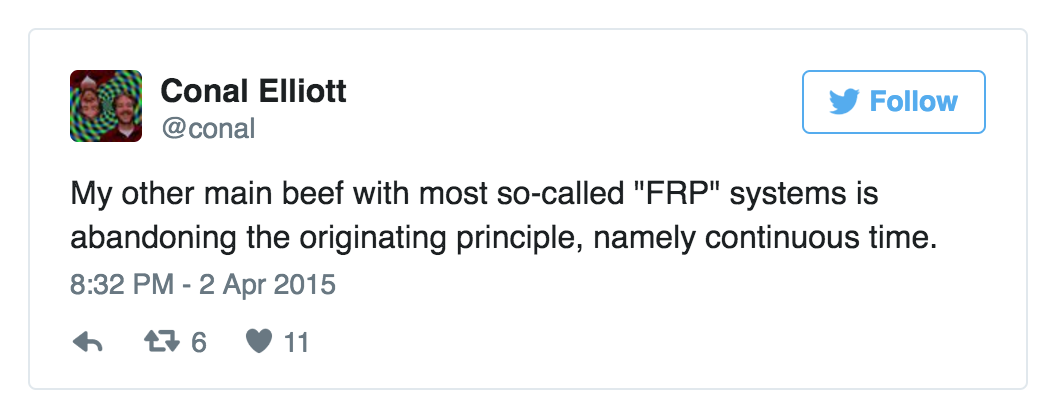
\includegraphics[scale=0.5]{img/not_frp1}
    \caption{Conal Eliott - dauguma bibliotekų iš tiesų nėra FRP, kaip jos teigia}
    \label{img:not_frp1}
\end{figure}

\begin{figure}[H]
    \centering
    
\includegraphics[scale=0.5]{img/not_frp2}
    \caption{Conal Eliott - dauguma bibliotekų iš tiesų nėra FRP, kaip jos teigia}
    \label{img:not_frp2}
\end{figure}

\begin{figure}[H]
    \centering
    
\includegraphics[scale=0.5]{img/not_frp3}
    \caption{Conal Eliott - dauguma bibliotekų iš tiesų nėra FRP, kaip jos teigia}
    \label{img:not_frp3}
\end{figure}

\begin{figure}[H]
    \centering
    
\includegraphics[scale=0.5]{img/not_frp4}
    \caption{Conal Eliott - dauguma bibliotekų iš tiesų nėra FRP, kaip jos teigia}
    \label{img:not_frp4}
\end{figure}

\begin{figure}[H]
    \centering
    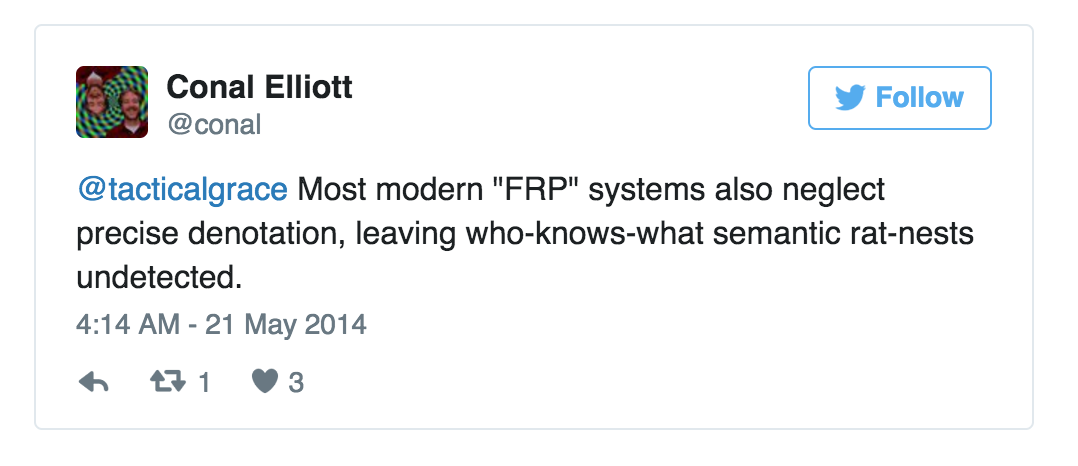
\includegraphics[scale=0.5]{img/not_frp5}
    \caption{Conal Eliott - dauguma bibliotekų iš tiesų nėra FRP, kaip jos teigia}
    \label{img:not_frp5}
\end{figure}

\begin{figure}[H]
    \centering
    
\includegraphics[scale=0.5]{img/not_frp6}
    \caption{Conal Eliott - dauguma bibliotekų iš tiesų nėra FRP, kaip jos teigia}
    \label{img:not_frp6}
\end{figure}

\begin{figure}[H]
    \centering
    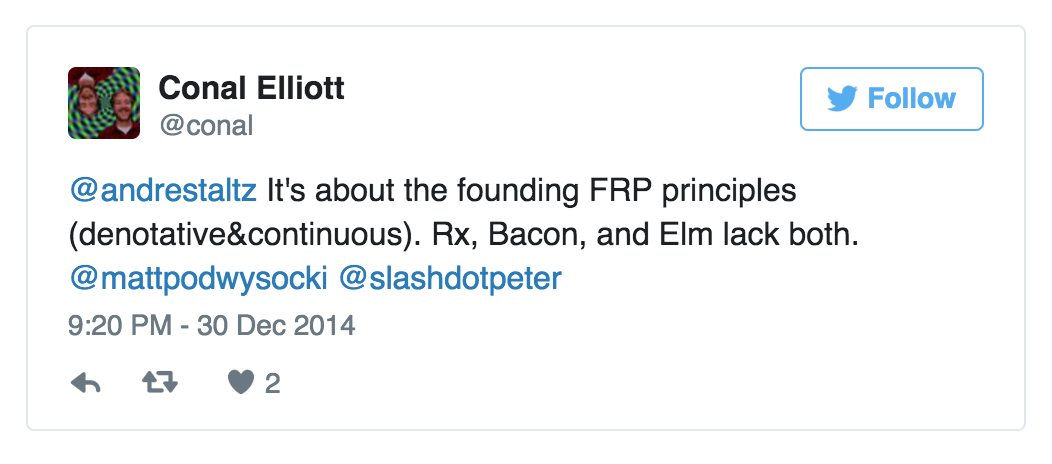
\includegraphics[scale=0.5]{img/not_frp7}
    \caption{Conal Eliott - dauguma bibliotekų iš tiesų nėra FRP, kaip jos teigia}
    \label{img:not_frp7}
\end{figure}

\section{Reaktyvaus programavimo bibliotekos Ruby kalboje}

\begin{figure}[H]
    \centering
    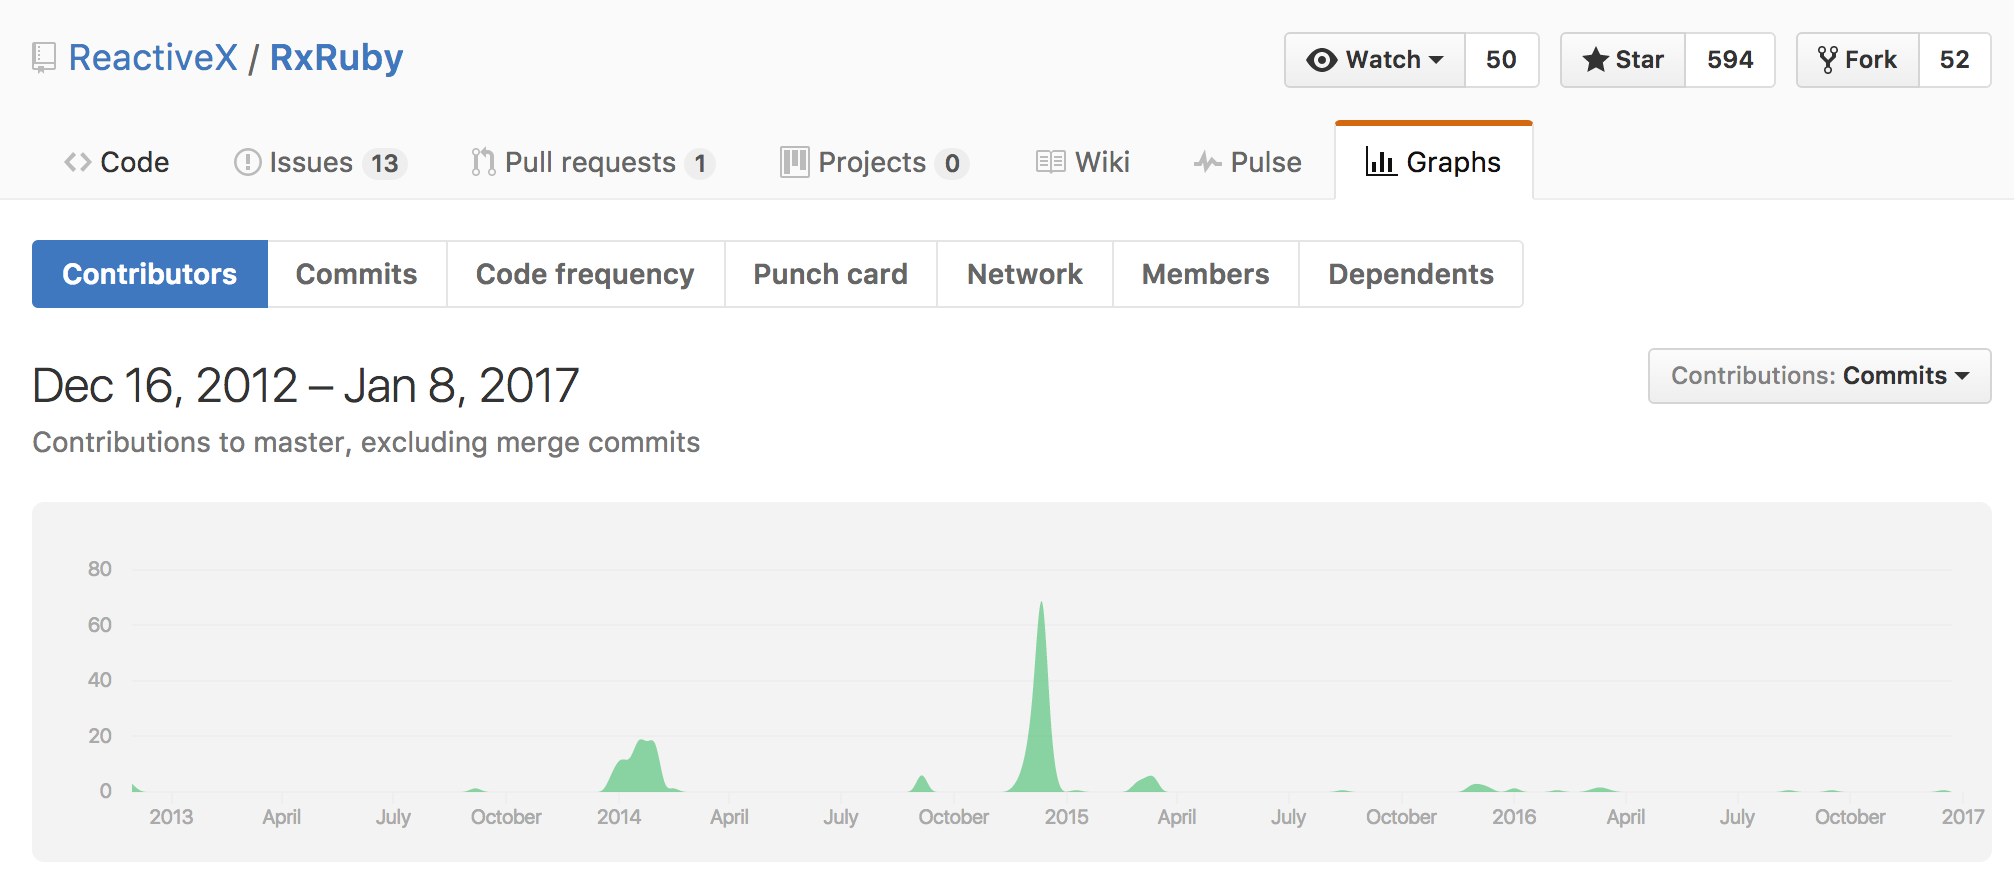
\includegraphics[scale=0.35]{img/rxruby}
    \caption{Reaktyvaus programavimo ``RxRuby'' biblioteka}
    \label{img:rxruby}
\end{figure}

\begin{figure}[H]
    \centering
    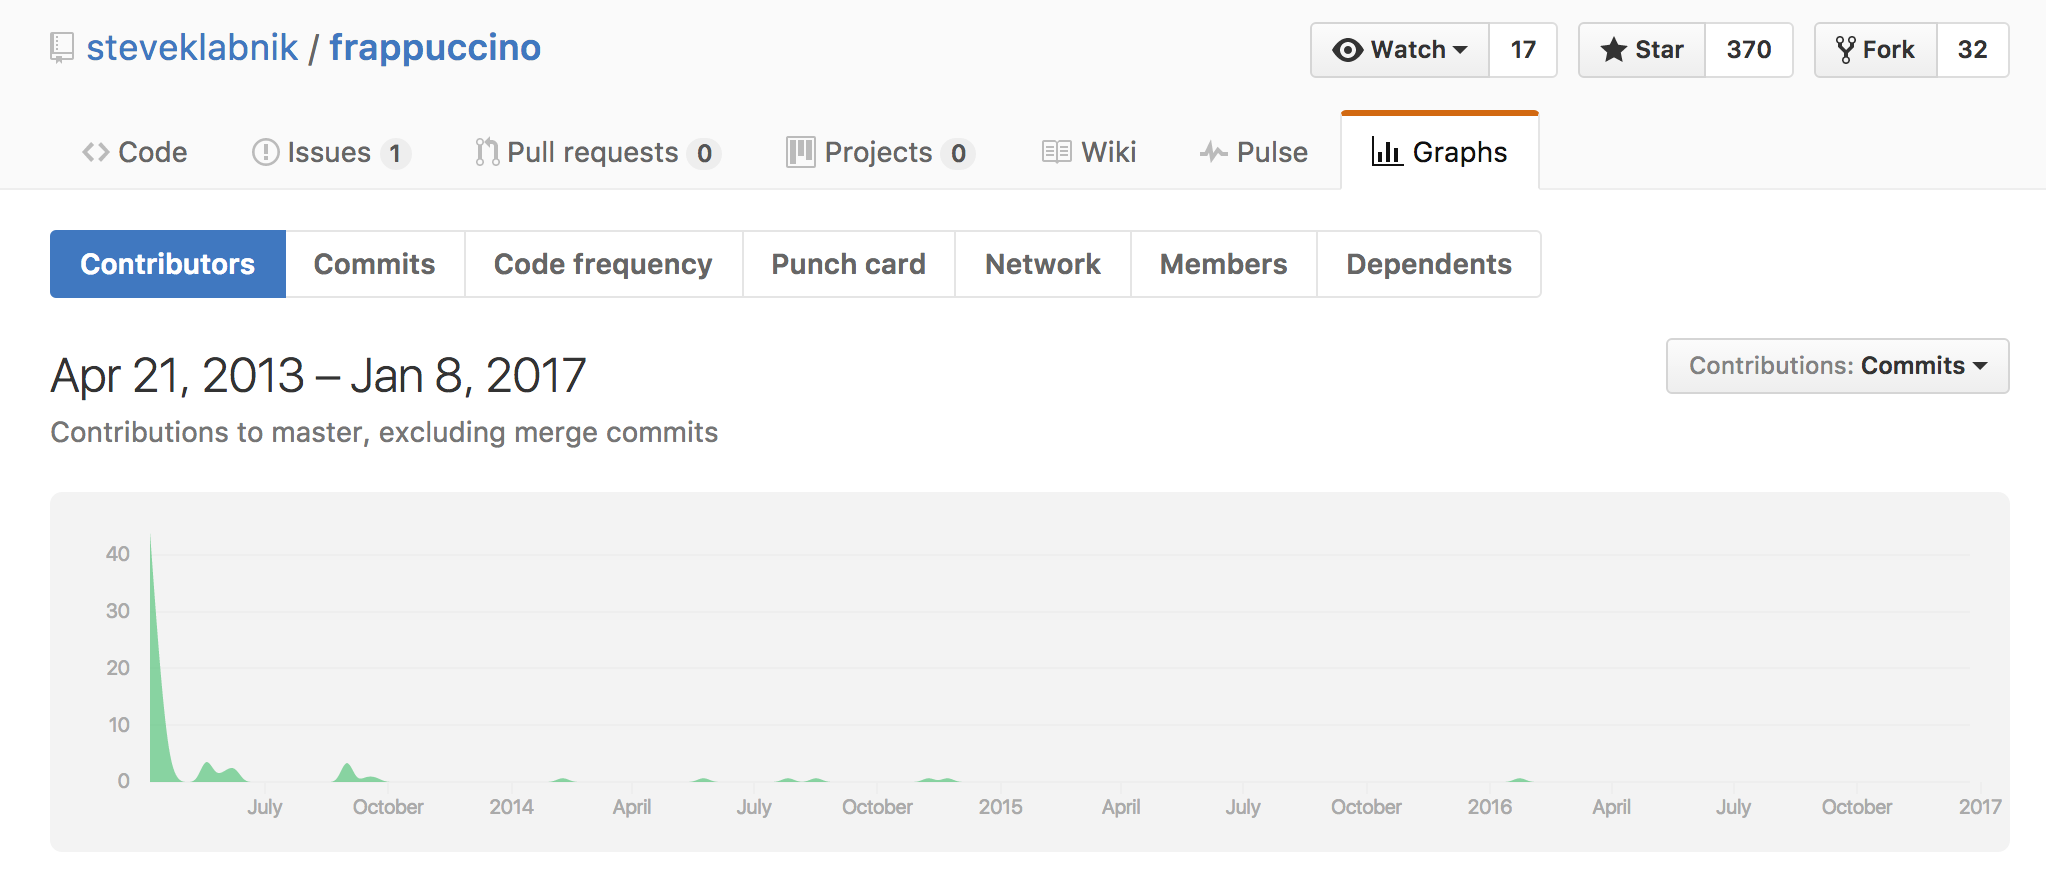
\includegraphics[scale=0.35]{img/frappuccino}
    \caption{Reaktyvaus programavimo ``Frappuccino'' biblioteka}
    \label{img:frappuccino}
\end{figure}

\section{Įvykių kaupimo bibliotekos Ruby kalboje}

\begin{figure}[H]
    \centering
    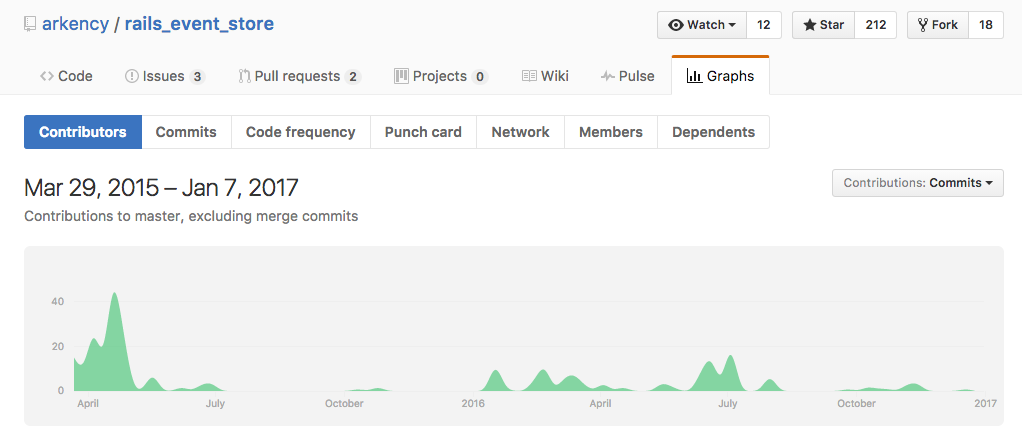
\includegraphics[scale=0.35]{img/rails_event_store}
    \caption{``RailsEventStore'' biblioteka įvykių kaupimo sistemoms kurti}
    \label{img:rails_event_store}
\end{figure}

\begin{figure}[H]
    \centering
    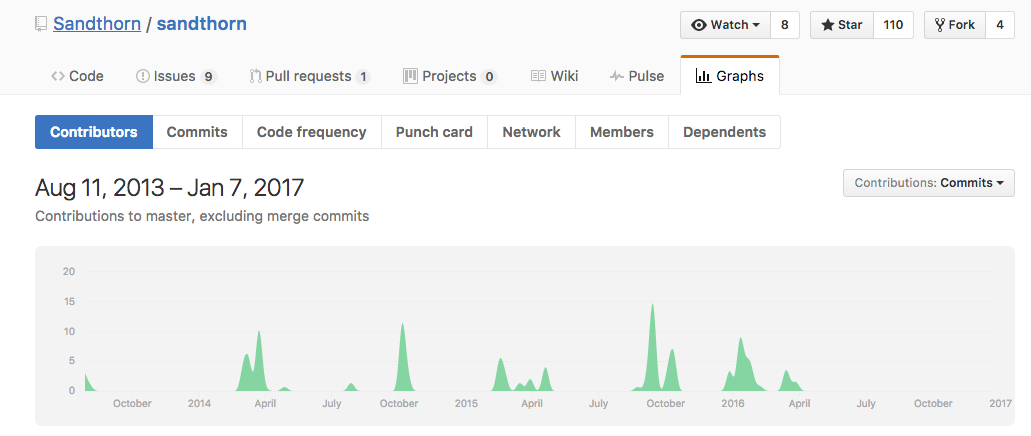
\includegraphics[scale=0.35]{img/sandthorn}
    \caption{``Sandthorn'' biblioteka įvykių kaupimo sistemoms kurti}
    \label{img:sandthorn}
\end{figure}

\begin{figure}[H]
    \centering
    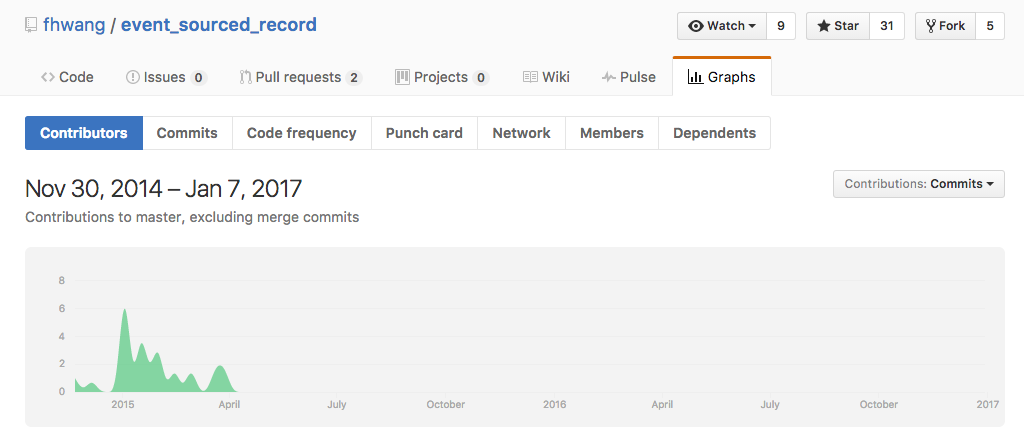
\includegraphics[scale=0.35]{img/event_sourced_record}
    \caption{``Event Sourced Record'' biblioteka įvykių kaupimo sistemoms kurti}
    \label{img:event_sourced_record}
\end{figure}

\end{document}
